\documentclass{article}



\usepackage{arxiv}

\usepackage[utf8]{inputenc} % allow utf-8 input
\usepackage[T1]{fontenc}    % use 8-bit T1 fonts
\usepackage{hyperref}       % hyperlinks
\usepackage{url}            % simple URL typesetting
\usepackage{booktabs}       % professional-quality tables
\usepackage{amsfonts}       % blackboard math symbols
\usepackage{nicefrac}       % compact symbols for 1/2, etc.
\usepackage{microtype}      % microtypography
\usepackage{lipsum}		% Can be removed after putting your text content
\usepackage{graphicx}
\usepackage{natbib}
\usepackage{doi}

\usepackage[dvipsnames]{xcolor}
\newcommand{\andy}[1]{\textcolor{blue}{\emph{#1}}}

\title{Could mass eccentricity explain the formation of orbits in wind turbines?}

%\date{September 9, 1985}	% Here you can change the date presented in the paper title
%\date{} 					% Or removing it

\author{ \href{https://orcid.org/0000-0000-0000-0000}{
\includegraphics[scale=0.06]{orcid.pdf}\hspace{1mm} Aljoscha Sander}\thanks{Use footnote for providing further information about author (webpage, alternative address)---\emph{not} for acknowledging funding agencies.} \\
	Energy and Sustainability Research Institute Groningen\\
	University of Groningen\\
	Groningen, the Netherlands \\
	\texttt{aljoscha.sander@rug.nl} \\
	%% examples of more authors
	\And
	\href{https://orcid.org/0000-0000-0000-0000}{
\includegraphics[scale=0.06]{orcid.pdf}\hspace{1mm} Andreas Haselsteiner} \\
	\texttt{a.haselsteiner@uni-bremen.de} \\
	\And
	Bas Holman \\
	\texttt{b.holman@outlook.com}\\
	%% Address \\
	%% \texttt{email} \\
	%% \And
	%% Coauthor \\
	%% Affiliation \\
	%% Address \\
	%% \texttt{email} \\
	%% \And
	%% Coauthor \\
	%% Affiliation \\
	%% Address \\
	%% \texttt{email} \\
}

% Uncomment to remove the date
%\date{}

% Uncomment to override  the `A preprint' in the header
%\renewcommand{\headeright}{Technical Report}
%\renewcommand{\undertitle}{Technical Report}
\renewcommand{\shorttitle}{Mass eccentricity in offshore wind turbines}

%%% Add PDF metadata to help others organize their library
%%% Once the PDF is generated, you can check the metadata with
%%% $ pdfinfo template.pdf
\hypersetup{
pdftitle={Could mass eccentricity explain the formation of orbits in wind turbines?},
pdfsubject={},
pdfauthor={Aljoscha Sander, Andreas Haselsteiner, Bas Holman},
pdfkeywords={First keyword, Second keyword, More},
}

\begin{document}
\maketitle

\begin{abstract}
\end{abstract}


% keywords can be removed
\keywords{First keyword \and Second keyword \and More}


\section{Introduction}
\label{sec:introduction}

Offshore wind is growing continuously and is on its way to become one of the pillars of green energy. Recent cost reductions in offshore wind (29 \%) have mostly been due to increasing turbine size \citep{irenaRenewablePowerGeneration2020}. Increasing turbine size and numbers, however, leads to increasing difficulties during installation: larger components are more difficult to handle and require more space on an installation vessel. Today, most turbines are installed component by component, including the blades, a process generally referred to as single blade installation \citep{jiangInstallationOffshoreWind2021}. Blades are installed utilizing a specialized tool, usually referred to as an installation yoke, that securely fastens the blade during craning operations. Once the blade reaches hub height, a guiding pin is used to land the blade's bolts in the corresponding holes in the rotor flange. During this operation, relative motion between the blade root and the rotor hub greatly hampers the secure landing of the blade in the rotor's flange. As these relative motions are driven by environmental loading on both the turbine and the blade, they are difficult to understand and even more to predict. 

In a measurement campaign during the installation of the offshore wind farm \textit{Trianel Windpark Borkum II} off the coast of Germany in the German Bight, the kinematics of blades and partially installed turbines were investigated \citep{sanderRelativeMotionSingle2020,  sanderMONITORINGOFFSHOREWIND2020, sanderOscillationsOffshoreWind2020}. These measurements revealed, that the partially installed turbines were displaying intricate patterns of motions — orbits — during single blade installation. A two-minute orbit captured during the installation of the wind park \textit{Trianel Windpark Borkum II} is shown in \autoref{fig:orbit}. These orbits show that amplitude and direction of tower top motion may occur swiftly and with large rates of change. It stands to reason that these orbits in turn influence the installation of blades and may even be responsible for an increase in installation difficulty.

\begin{figure}[ht!]
    \centering
    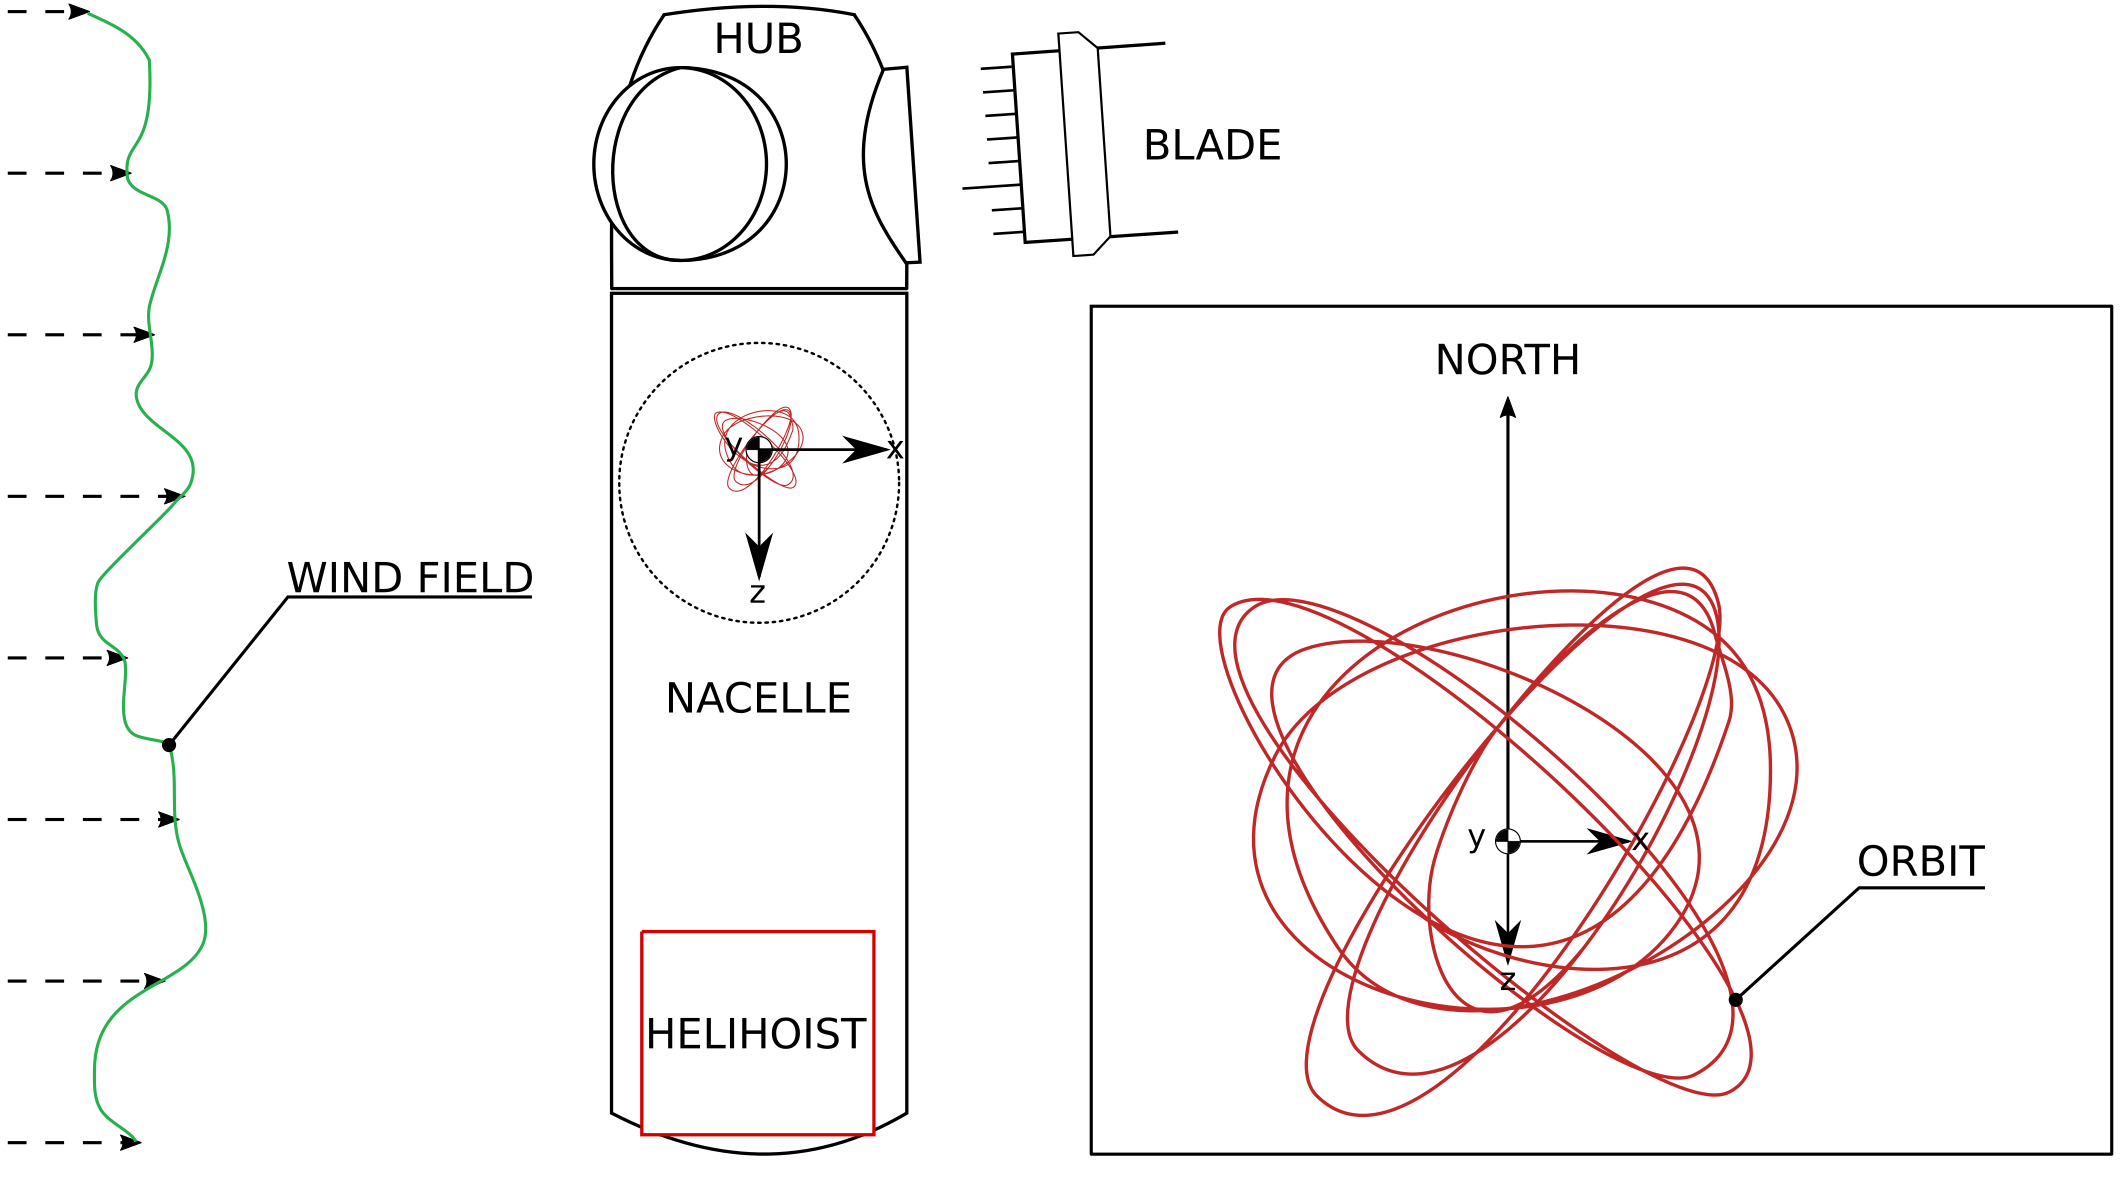
\includegraphics[width=0.7\linewidth]{manuscript/figures/installation_alt2.png}
    \caption{Formation of orbits as observed during the installation of the offshore wind park \textit{Trianel Windpark Borkum II}. Note: the orbits are not to scale to enhance visibility.}
    \label{fig:orbit}
\end{figure}

Several mechanisms may in theory explain the formation of orbits. In this paper, we present a coupling mechanism that intrinsically leads to the formation of orbits in a cantilevered beam. 

In this paper, we focus on one specific state of an offshore wind turbine during installation: the hammerhead configuration. In this configuration, the foundation, transition piece, tower, and nacelle have already been installed, and the next installation step would be the installation of the first blade. In this configuration, the turbine is top heavy and, due to the nacelle's and rotor's weight, also nose-heavy. In the case of the turbines installed at \textit{Trianel Windpark Borkum II}, the centre of gravity of the nacelle is approximately 0.3 m shifted towards the rotor with respect to the tower axis. \autoref{fig:loading} depicts the hammerhead configuration as well as the simplified mechanical system derived to investigate the behaviour of partially installed turbines during installation. 

\begin{figure}[ht!]
    \centering
    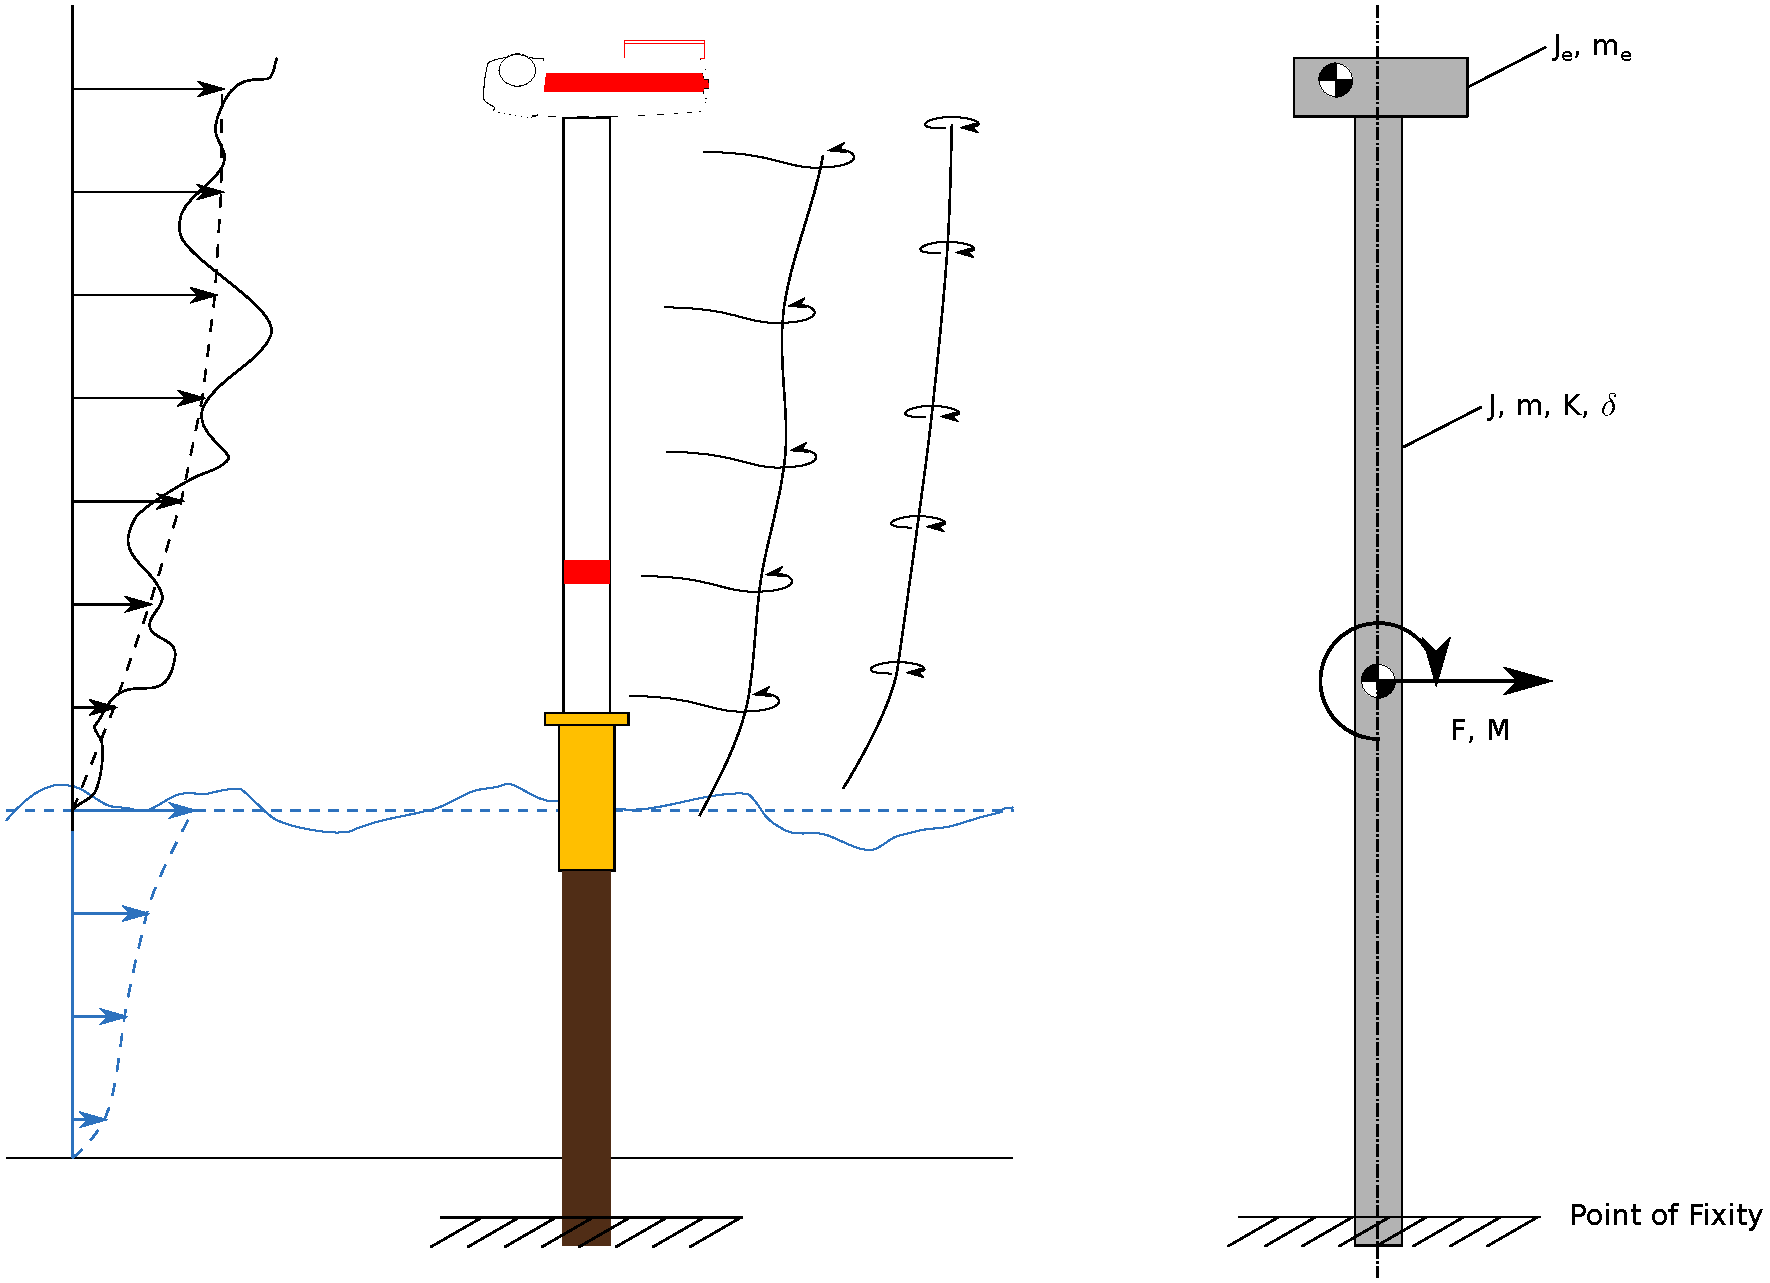
\includegraphics[width=0.7\linewidth]{manuscript/figures/loading_3.pdf}
    \caption{Hammerhead configuration (left) and simplified mechanical model of the hammerhead configuration (right).}
    \label{fig:loading}
\end{figure}

This system represents a cantilevered beam with an eccentric mass at the free end. We hypothesize that the inertia of the eccentric mass leads to torsion of the cantilevered beam if the tower vibrates transversally. Twisting the tower has two effects: a) the circular motion of the eccentric mass has a component perpendicular to the initial direction of motion, and thus momentum from that circular motion transfers into the perpendicular direction. b) twisting the tower leads to a torsional oscillation of the eccentric mass around the tower axis. The torsional motion of the eccentric mass in illustrated in \autoref{fig:kinematics}.

\clearpage

\begin{figure}[ht!]
    \centering
    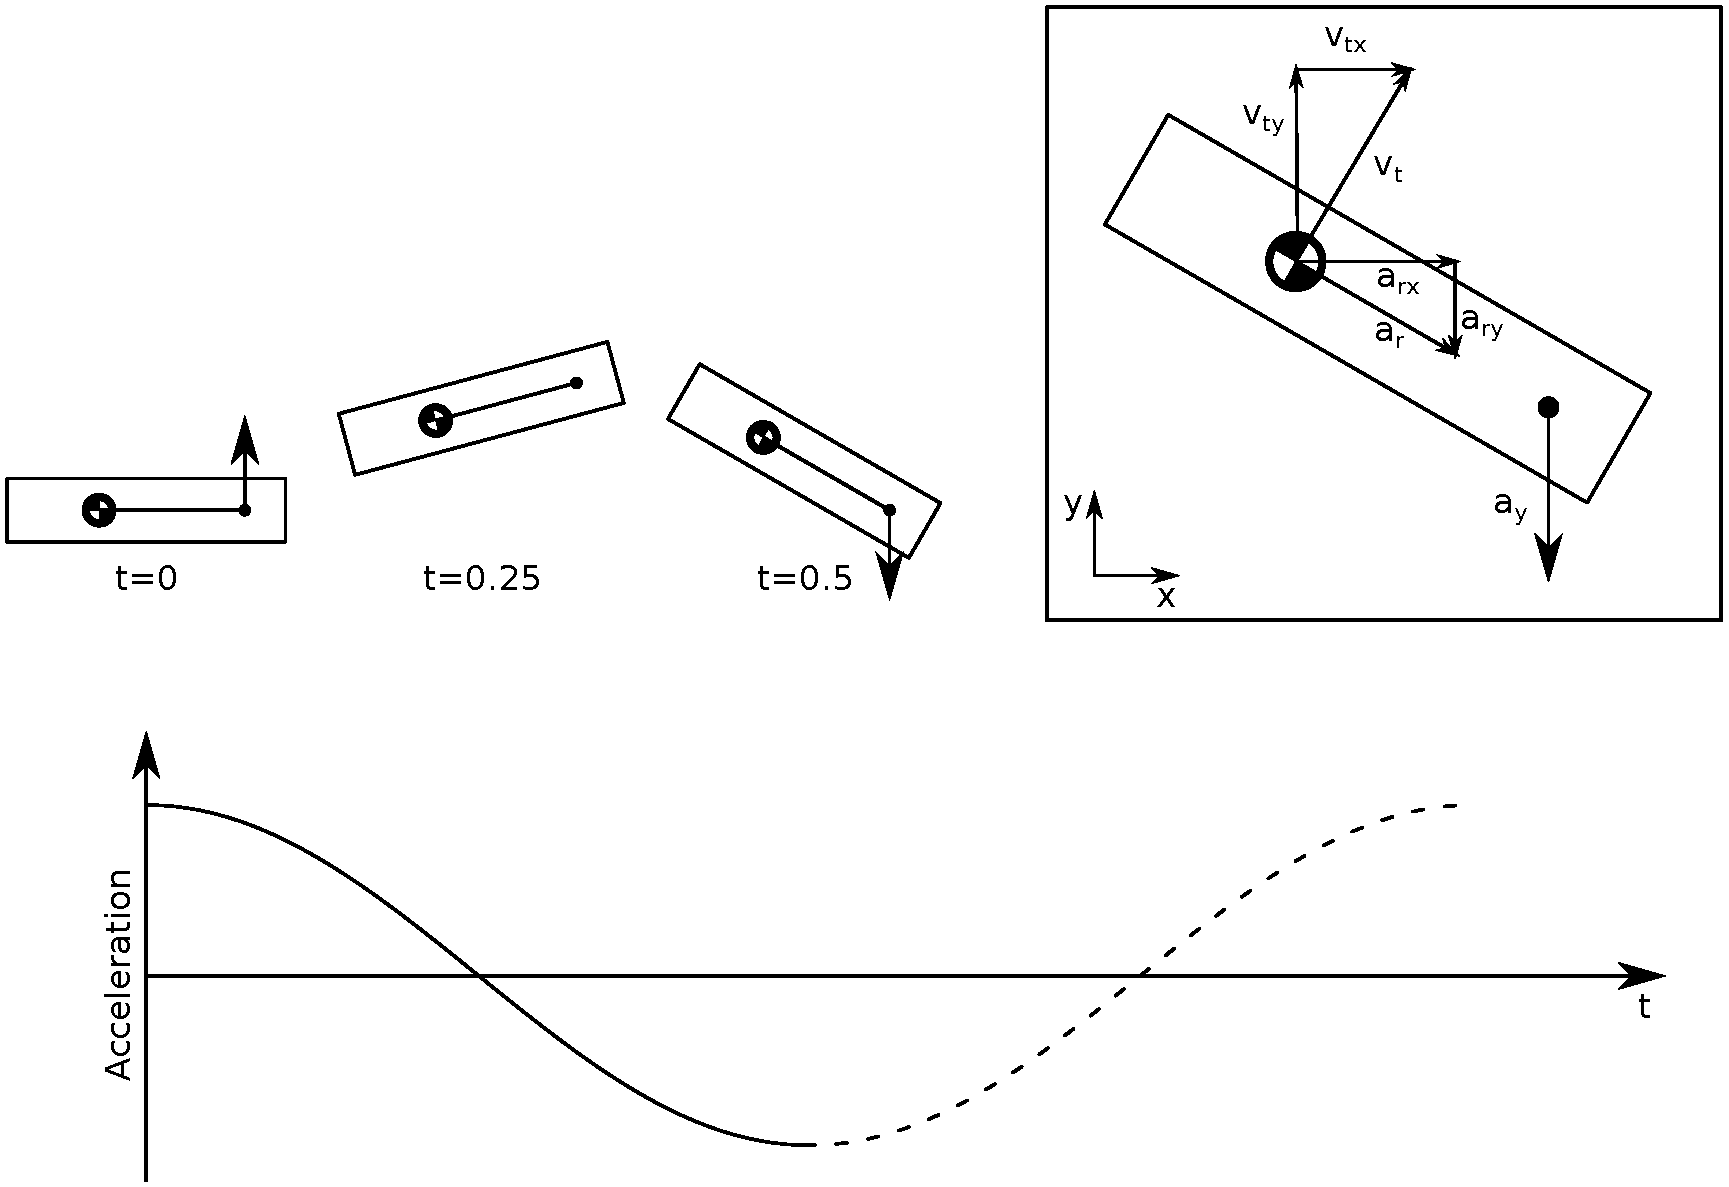
\includegraphics[width=0.7\linewidth]{manuscript/figures/kinematics.pdf}
    \caption{Simplified kinematics of an eccentric mass undergoing harmonic oscillations.}
    \label{fig:kinematics}
\end{figure}

The paper is subdivided into four sections: first, results from a table-top experiment (\autoref{sec:experiment}), capable of reproducing the torsional coupling, are shown. A section on finite-element-simulations (\autoref{sec:simulations}) of a comparable system follows. Finally, a discrete system of differential equations (\autoref{sec:3dof}) is presented. The final section (\autoref{sec:discussion}) discusses the effect and the shortcomings of the presented approaches and discusses implications for future research into the topic. 

\clearpage

\section{Cantilever experiment}
\label{sec:experiment}

\subsection{Experimental Setup}

As a first proof of concept, we built a table-top experiment that allows us to demonstrate the effect of an eccentric mass on the vibration of a cantilevered beam. As a beam, we chose a wooden rod (massive beech, 0.006 m diameter) with a free length of 0.7 m. At the free end of the rod, we placed a 3D-printed lever that allowed us to add M8 bolts (0.028 m length, 0.0129 kg) to control the amount of eccentric mass. Lever length was 0.082 m weighing a total of XX kg. A second rod made of fibre glass (diameter 0.008 m) was placed next to the cantilevered beam. \autoref{fig:setup} shows the experimental setup. The second rod was used to displace the cantilevered beam from its resting position  by pulling the cantilevered beam towards the second rod using a thin thread. The initial displacement of the top of the rod was 0.135 m and three different masses (no bolts, two bolts, four bolts) were tested in the experiment. To release the cantilevered beam from it initial, displaced position, the thread set on fire using a lighter. While this release mechanism seems somewhat archaic, it ensures that no external torque is added to the system upon release. For each mass, the experiment was repeated three times. A MEMS-based inertial measurement unit (MPU 9255, InvenSense TDK, Tokyo, Japan) placed on top of the cantilevered beam measured linear acceleration and angular velocity with a sampling rate of 100 Hz. Measurements were recorded using a Raspberry Pi 400 and a custom written python script. All raw data is available at zenodo. 

\begin{figure}[ht!]
    \centering
    \includegraphics[width=0.5\linewidth]{manuscript/figures/setup.png}
    \caption{Experimental setup}
    \label{fig:setup}
\end{figure}

Results are post-processed using a Jupyter Notebook and Python3. The Jupyter Notebook is available here. 

First, obtained accelerations in fore-aft and side-side direction are resampled to 50 Hz using linear interpolation. 

As the data is indexed by the time of the recording, the time series of each experiment have to be normalized to enable comparison of the different time series. The first peak in the fore-aft acceleration signal in each recorded experiment serves as a normalization time stamp; Each signal is cropped, such that it starts 0.5 s prior to the first peak and last for 120 s. 

Following time normalization, the data is filtered by applying a Butterworth high-pass filter with a cut-off frequency of 0.5 Hz, order 11 and padding of 25 s to remove any transient effects. The filter is applied forwards and backwards in time to remove any frequency response (phase delay). Afterwards, the accelerations and the angular velocities are integrated using a second order trapez type integration, yielding the velocity vector of the rod's tip and the torsion angle of the rod. To obtain the displacement vector, the velocity vector is filtered again with the same Butterworth filter, integrated again and finally both torsion angle and displacement vector are filtered one last time with the same Butterworth filter.

To compare experimental measurements with finite element simulations and the 3-DoF model, the experimental results must be normalized to remove the influence of damping from the observed orbits. Therefore, the observed decay in amplitude over time is estimated using an exponential function of the following form:

\begin{equation}
    A = A_0 e ^ {\gamma t} + a
\end{equation}

Where $A_0$ is the initial amplitude, $\gamma$ is the damping coefficient and $a$ is a constant offset to account for the finite time series. To obtain orbits free of damping, the displacement vector is scaled by the exponential decay function. 

\subsection{Experimental Results}

\autoref{fig:low-mass}, \autoref{fig:medium-mass} and \autoref{fig:high-mass} each show the observed accelerations, the angular velocity and the absolute acceleration in the fore-aft-side-side plane as well as the corresponding orbits

\textbf{ToDo}

\begin{itemize}
    \item normalize time with eigenfrequencies? -> comparability of the time series would be enhanced
    \item draw bas' drawings
\end{itemize}

%%%
% Low mass
%%%

\begin{figure*}[ht]

    \centering
    \begin{subfigure}[b]{0.45\textwidth}
        \centering
        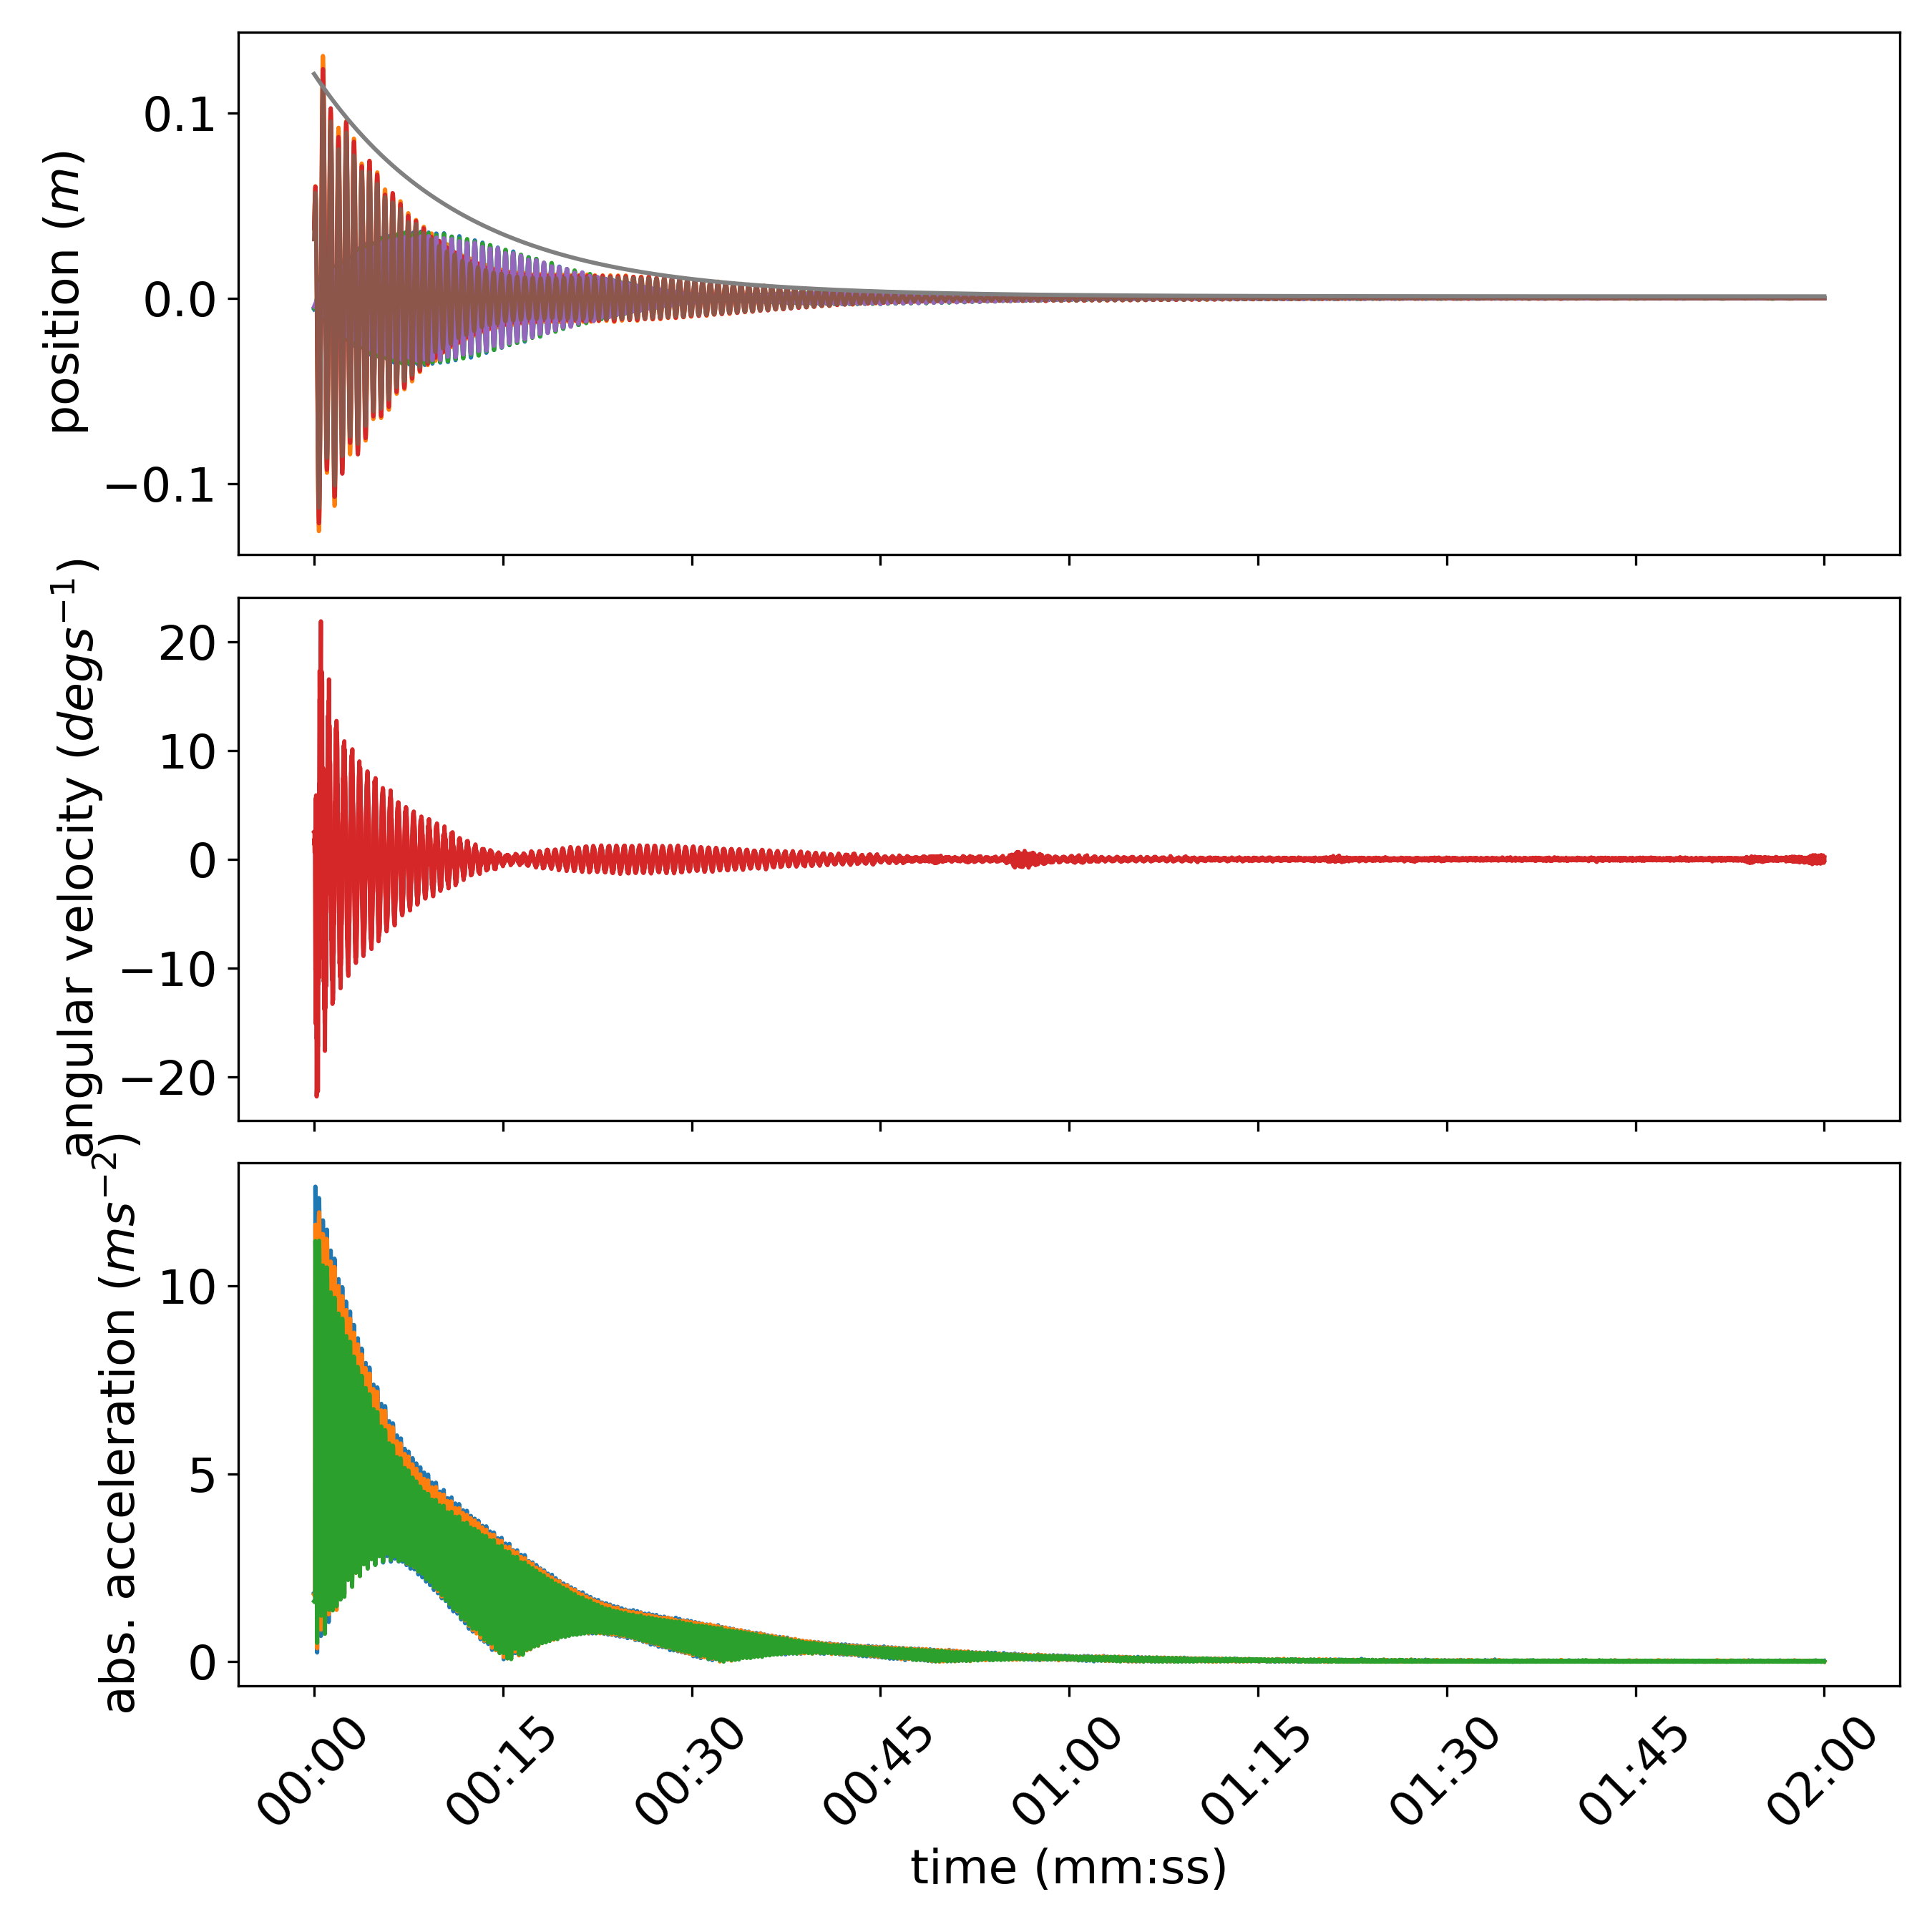
\includegraphics[width=\textwidth]{results/experiment/low_mass_acceleration.png}
        \caption{}
        % \caption{Scatter diagram for mean deflection $d_{10}$ and significant wave height $H_{S10}$. The linear fit is shown as a blue line.}
        \label{fig:low-mass:acc}
    \end{subfigure}
    \begin{subfigure}[b]{0.45\textwidth}
        \centering
        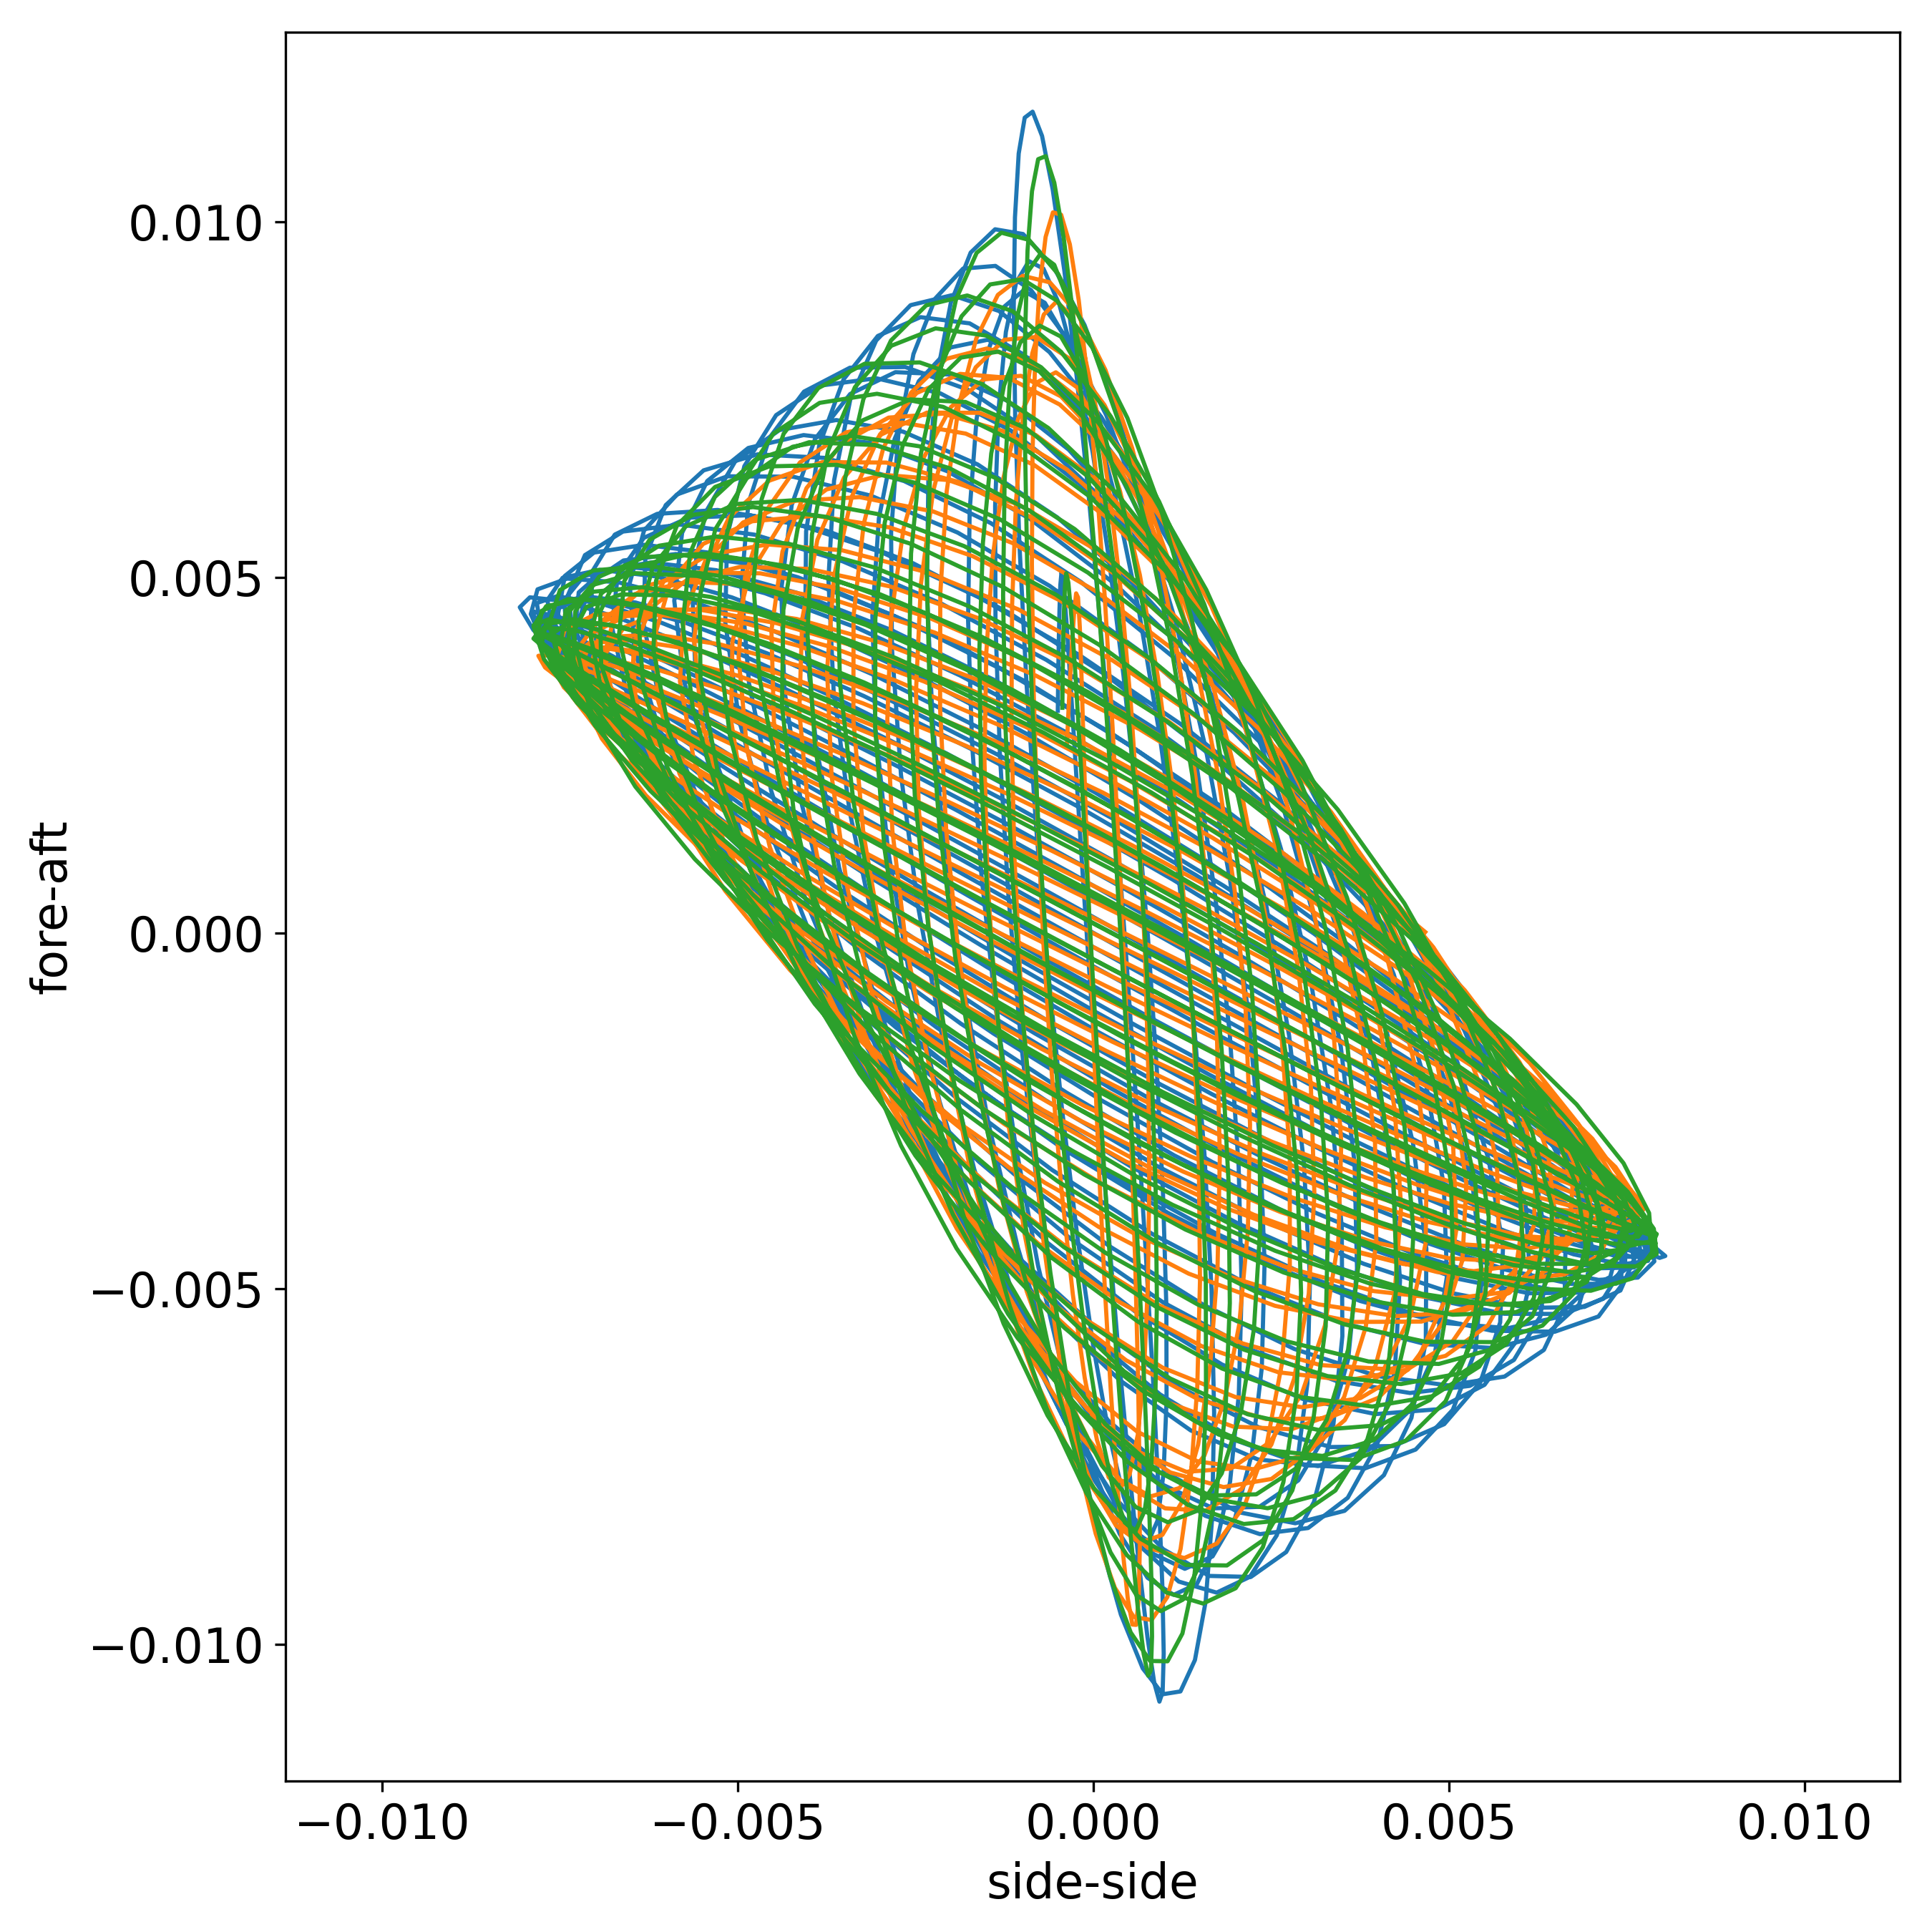
\includegraphics[width=\textwidth]{results/experiment/low_mass_orbit.png}
        \caption{}
        % \caption{Scatter diagram for mean deflection $d_{10}$ and significant wave height $H_{S10}$. The linear fit is shown as a blue line.}
        \label{fig:low-mass:orbit}
    \end{subfigure}
    
    \caption{Lissajous figures (orbits) for three different eccentric masses. \andy{[What are top's masses and moment of inertias of these configurations?]}}
    \label{fig:low-mass}
\end{figure*}

%%%
% medium mass
%%%

\begin{figure*}

    \centering
    \begin{subfigure}[b]{0.45\textwidth}
        \centering
        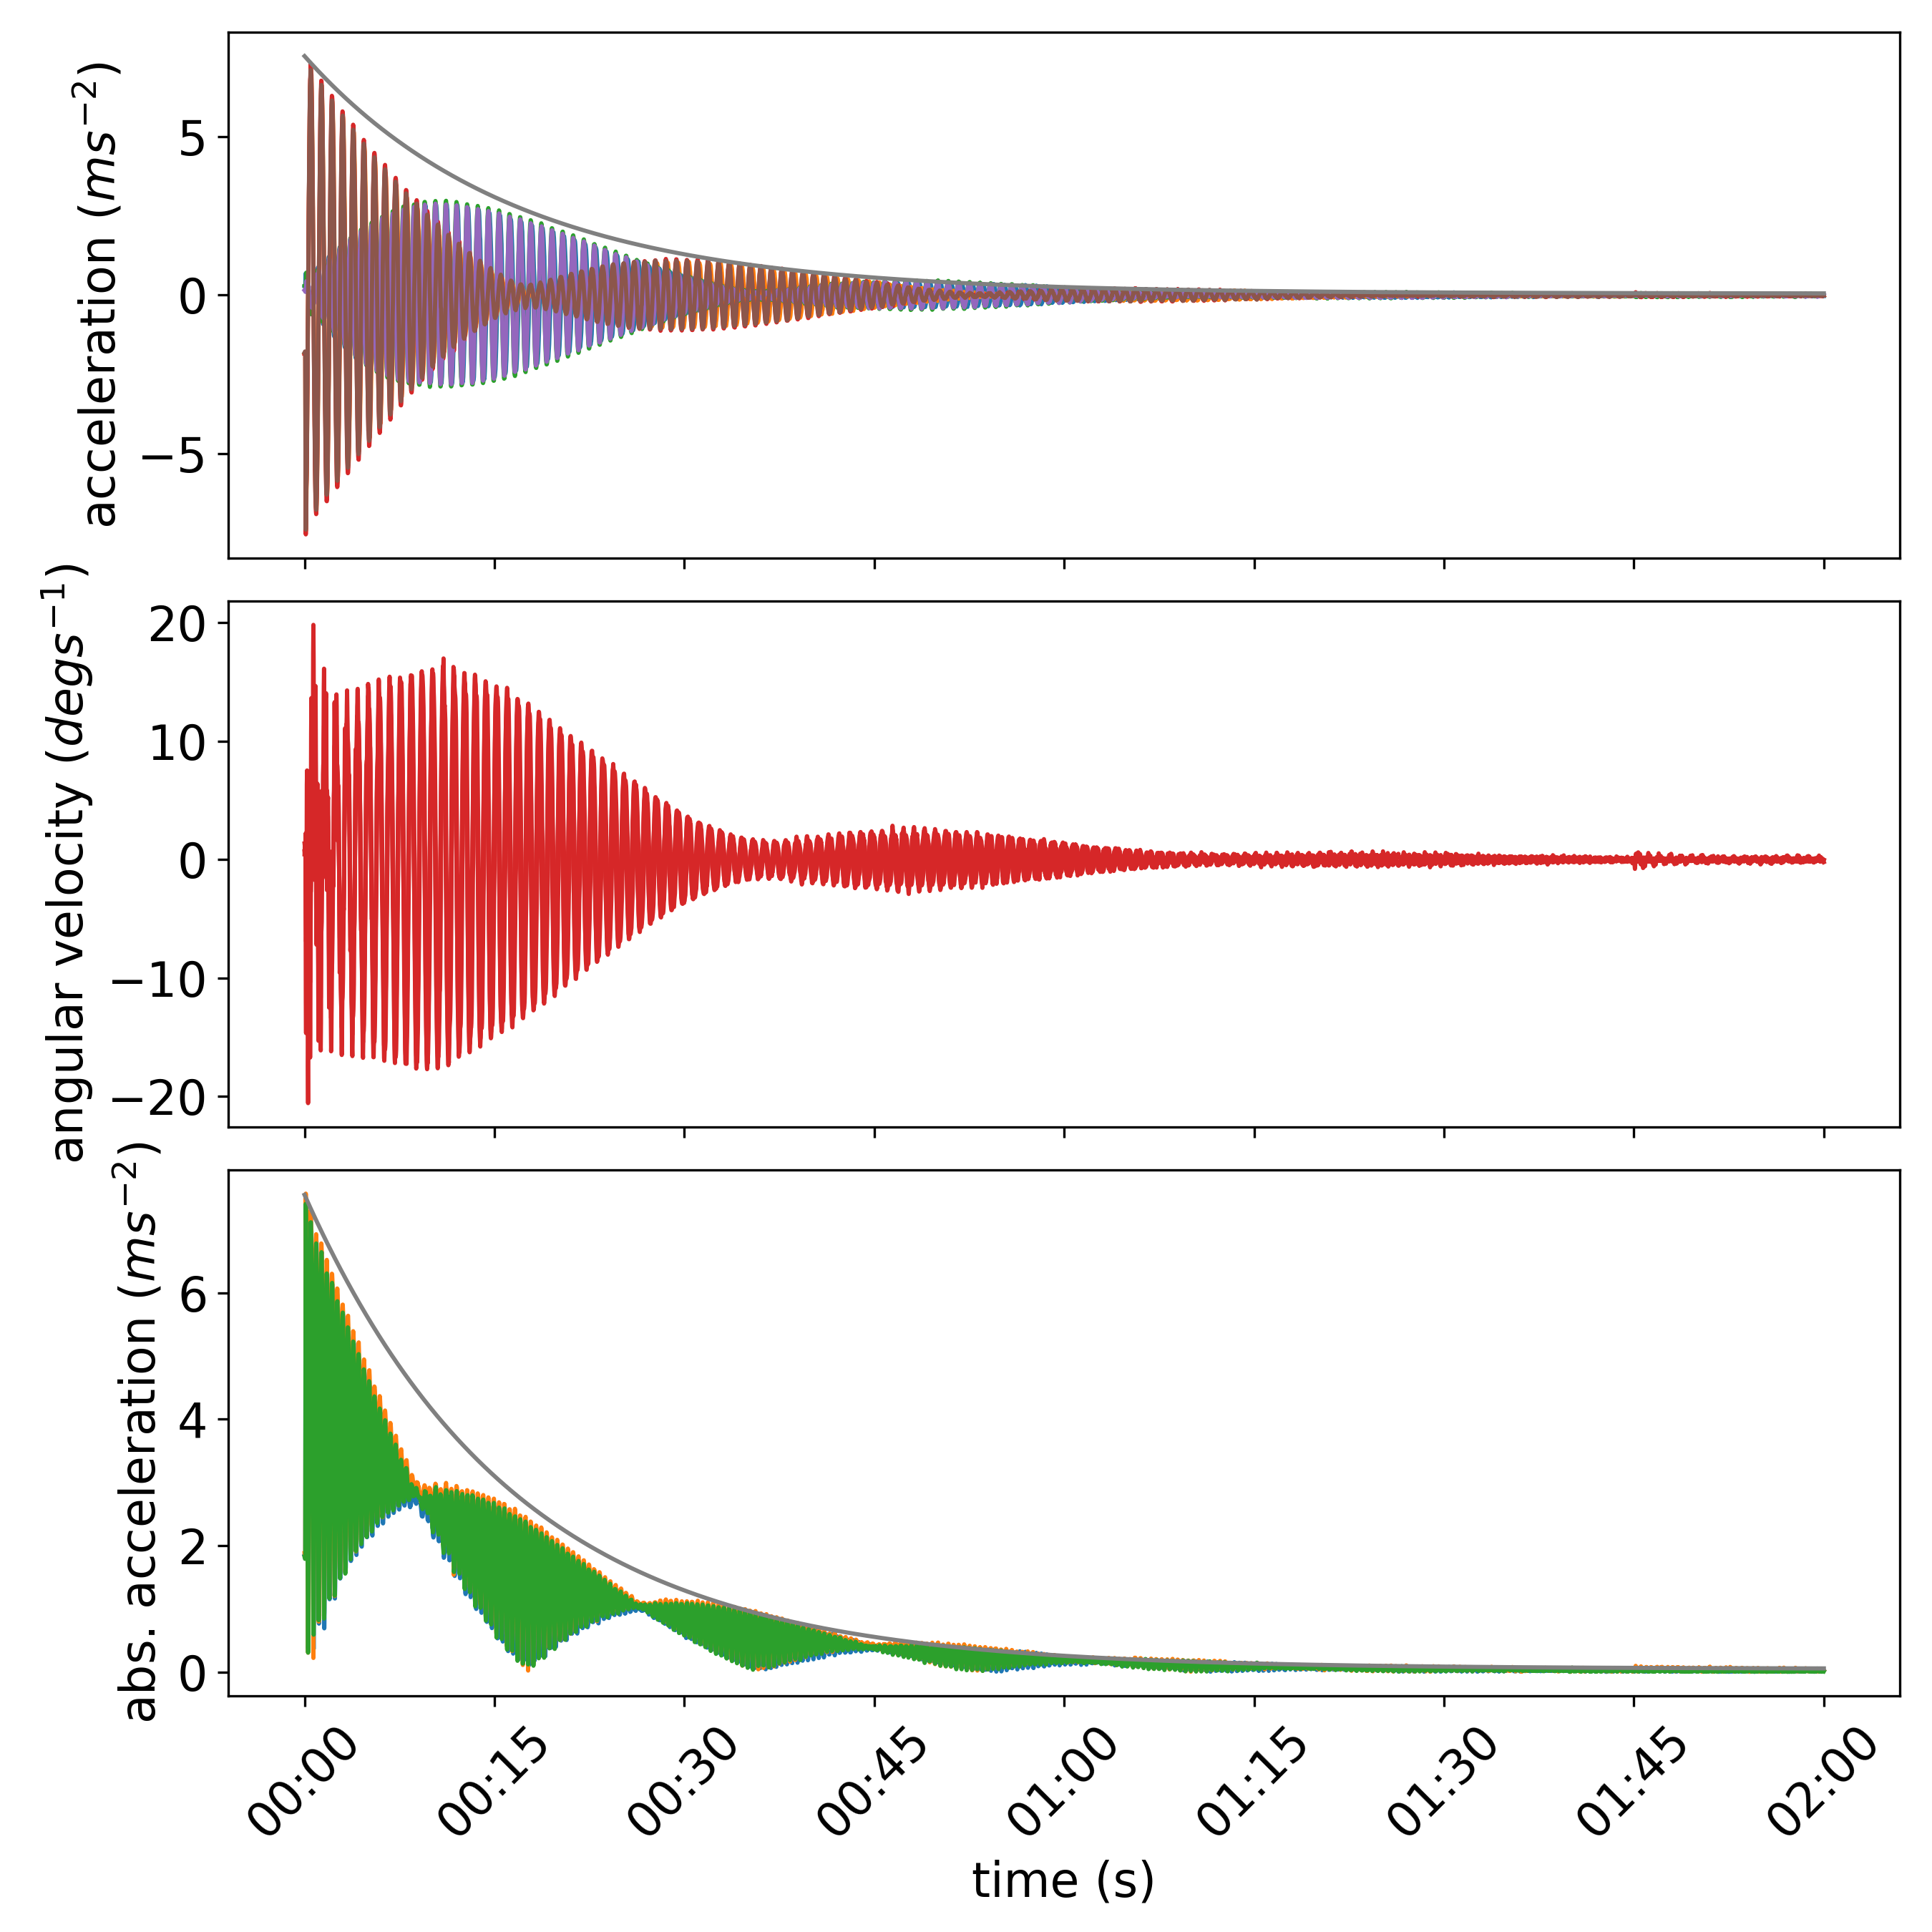
\includegraphics[width=\textwidth]{results/experiment/medium_mass_acceleration.png}
        \caption{}
        % \caption{Scatter diagram for mean deflection $d_{10}$ and significant wave height $H_{S10}$. The linear fit is shown as a blue line.}
        \label{fig:medium-mass:acc}
    \end{subfigure}
    \begin{subfigure}[b]{0.45\textwidth}
        \centering
        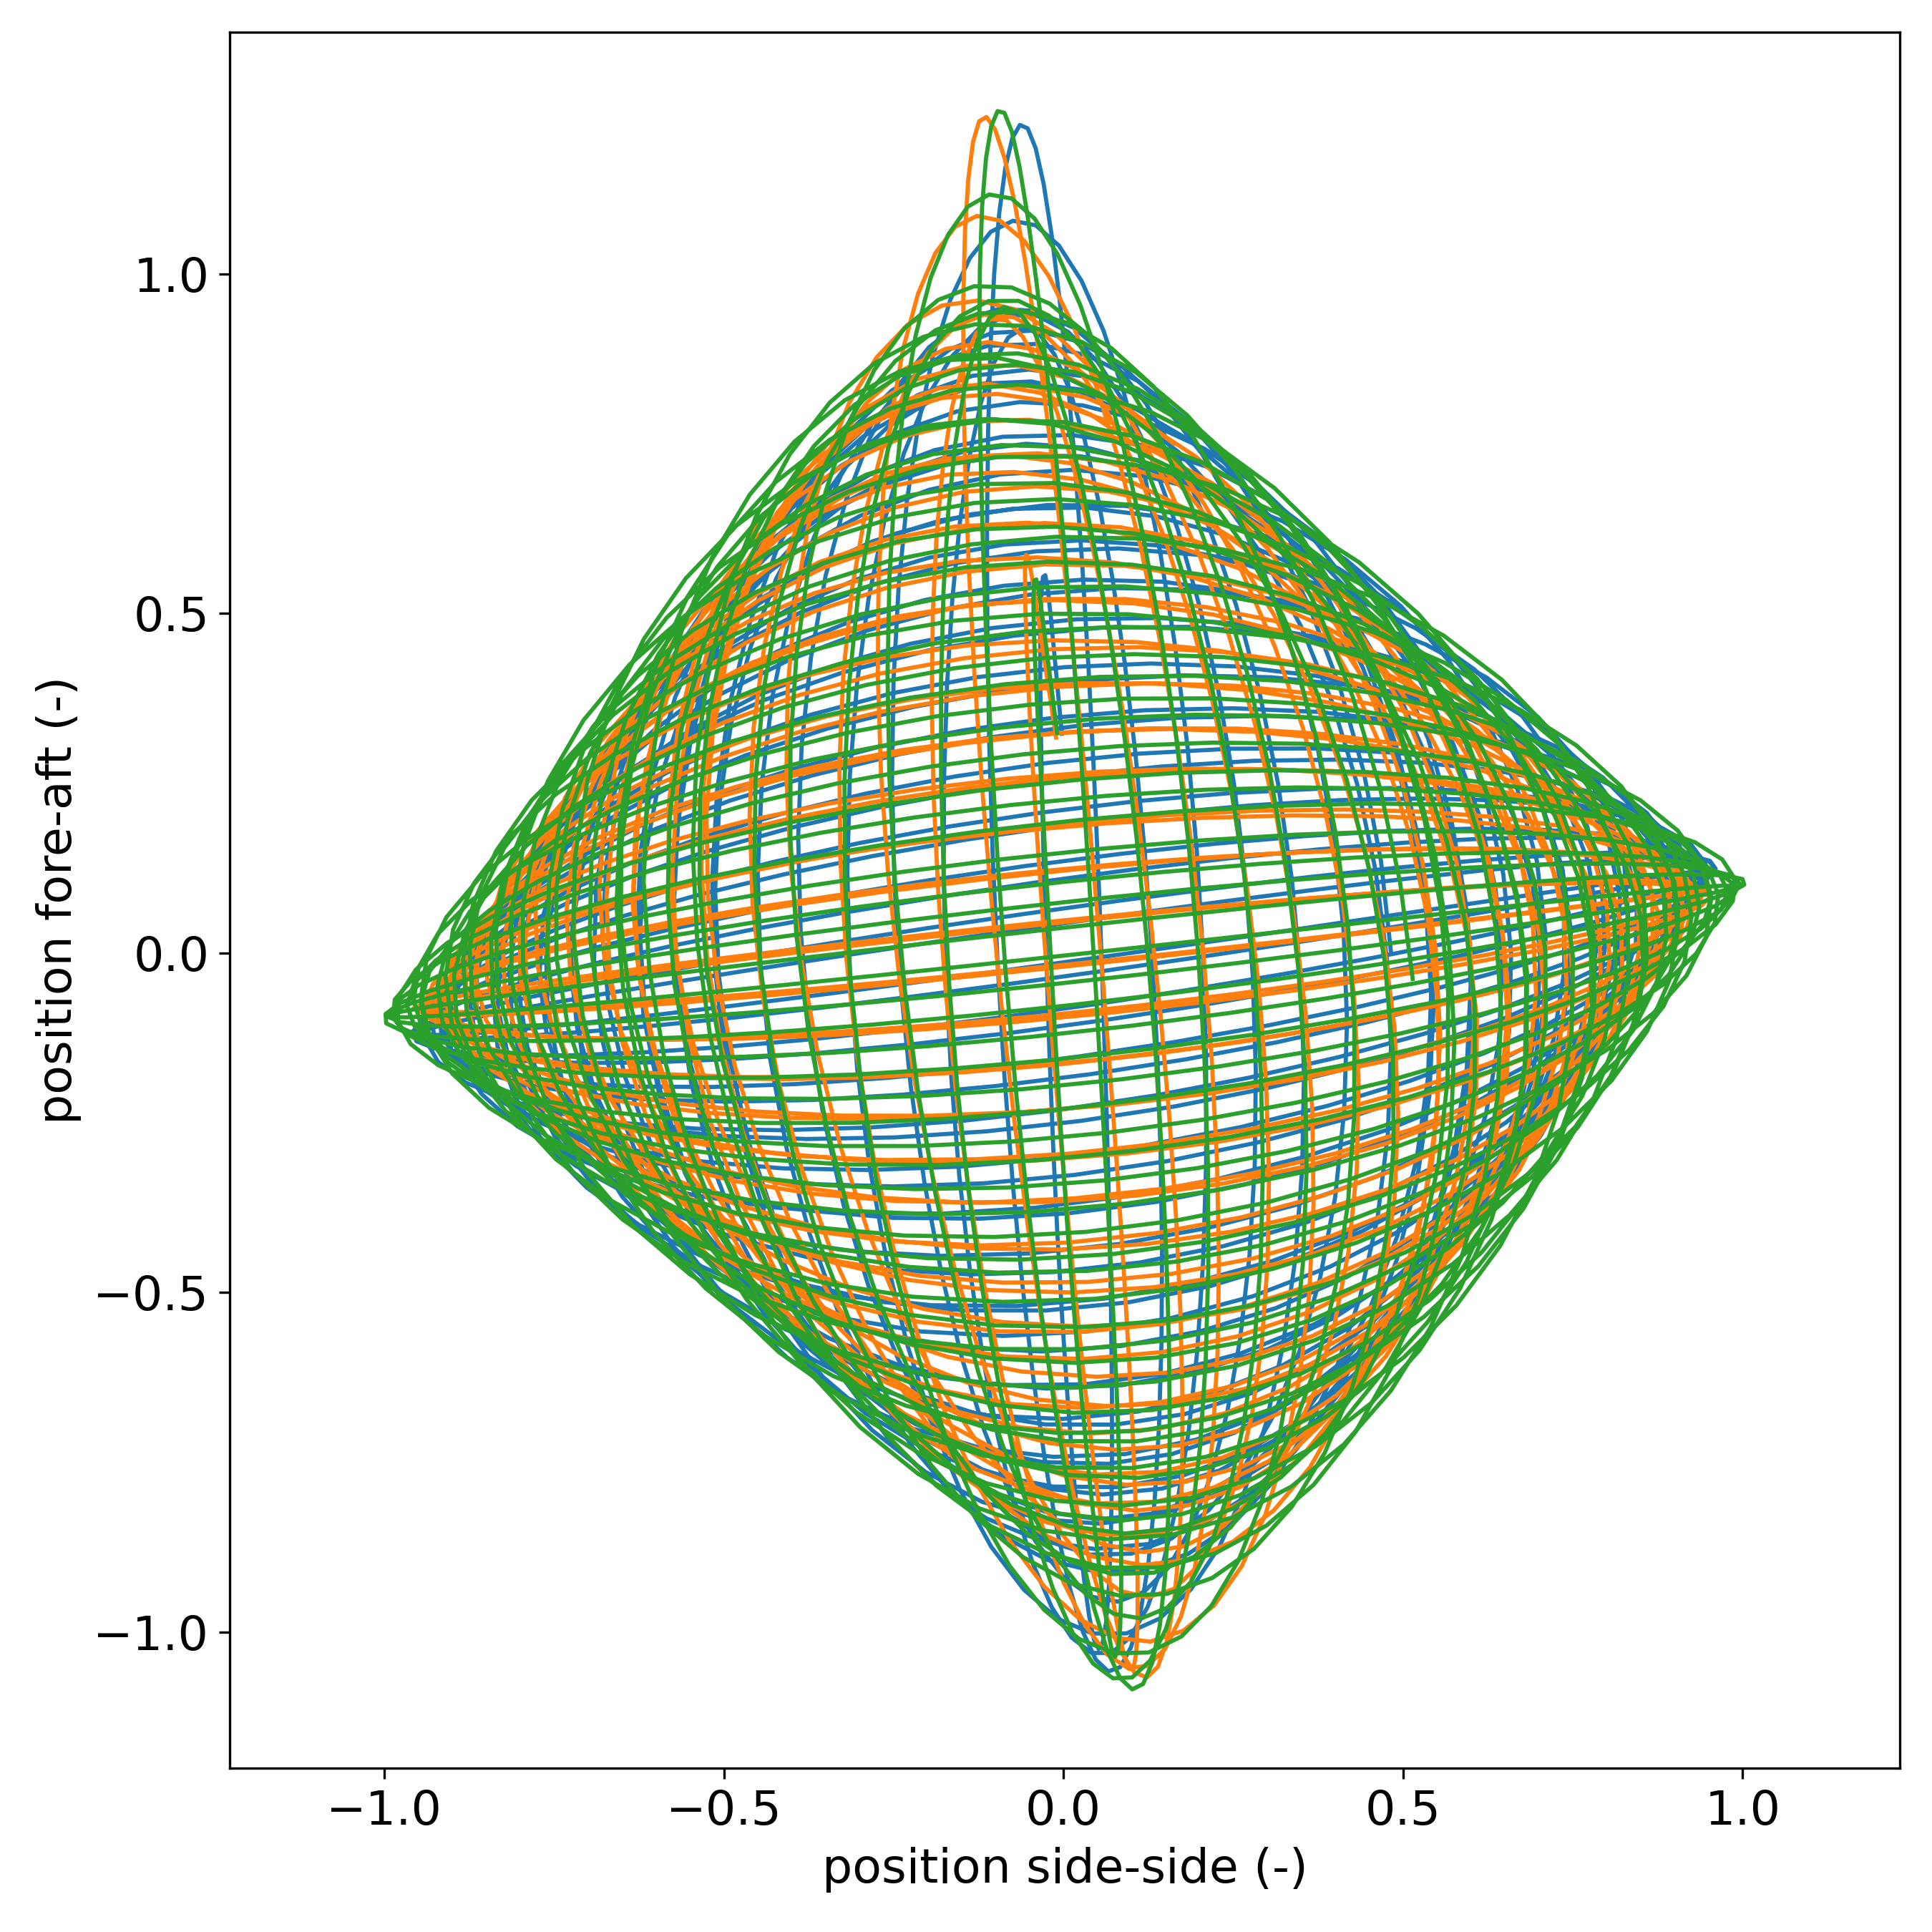
\includegraphics[width=\textwidth]{results/experiment/medium_mass_orbit.png}
        \caption{}
        % \caption{Scatter diagram for mean deflection $d_{10}$ and significant wave height $H_{S10}$. The linear fit is shown as a blue line.}
        \label{fig:medium-mass:orbit}
    \end{subfigure}
    
    \caption{Lissajous figures (orbits) for three different eccentric masses. \andy{[What are top's masses and moment of inertias of these configurations?]}}
    \label{fig:medium-mass}
\end{figure*}

%%%
% High mass
%%%

\begin{figure*}

    \centering
    \begin{subfigure}[b]{0.45\textwidth}
        \centering
        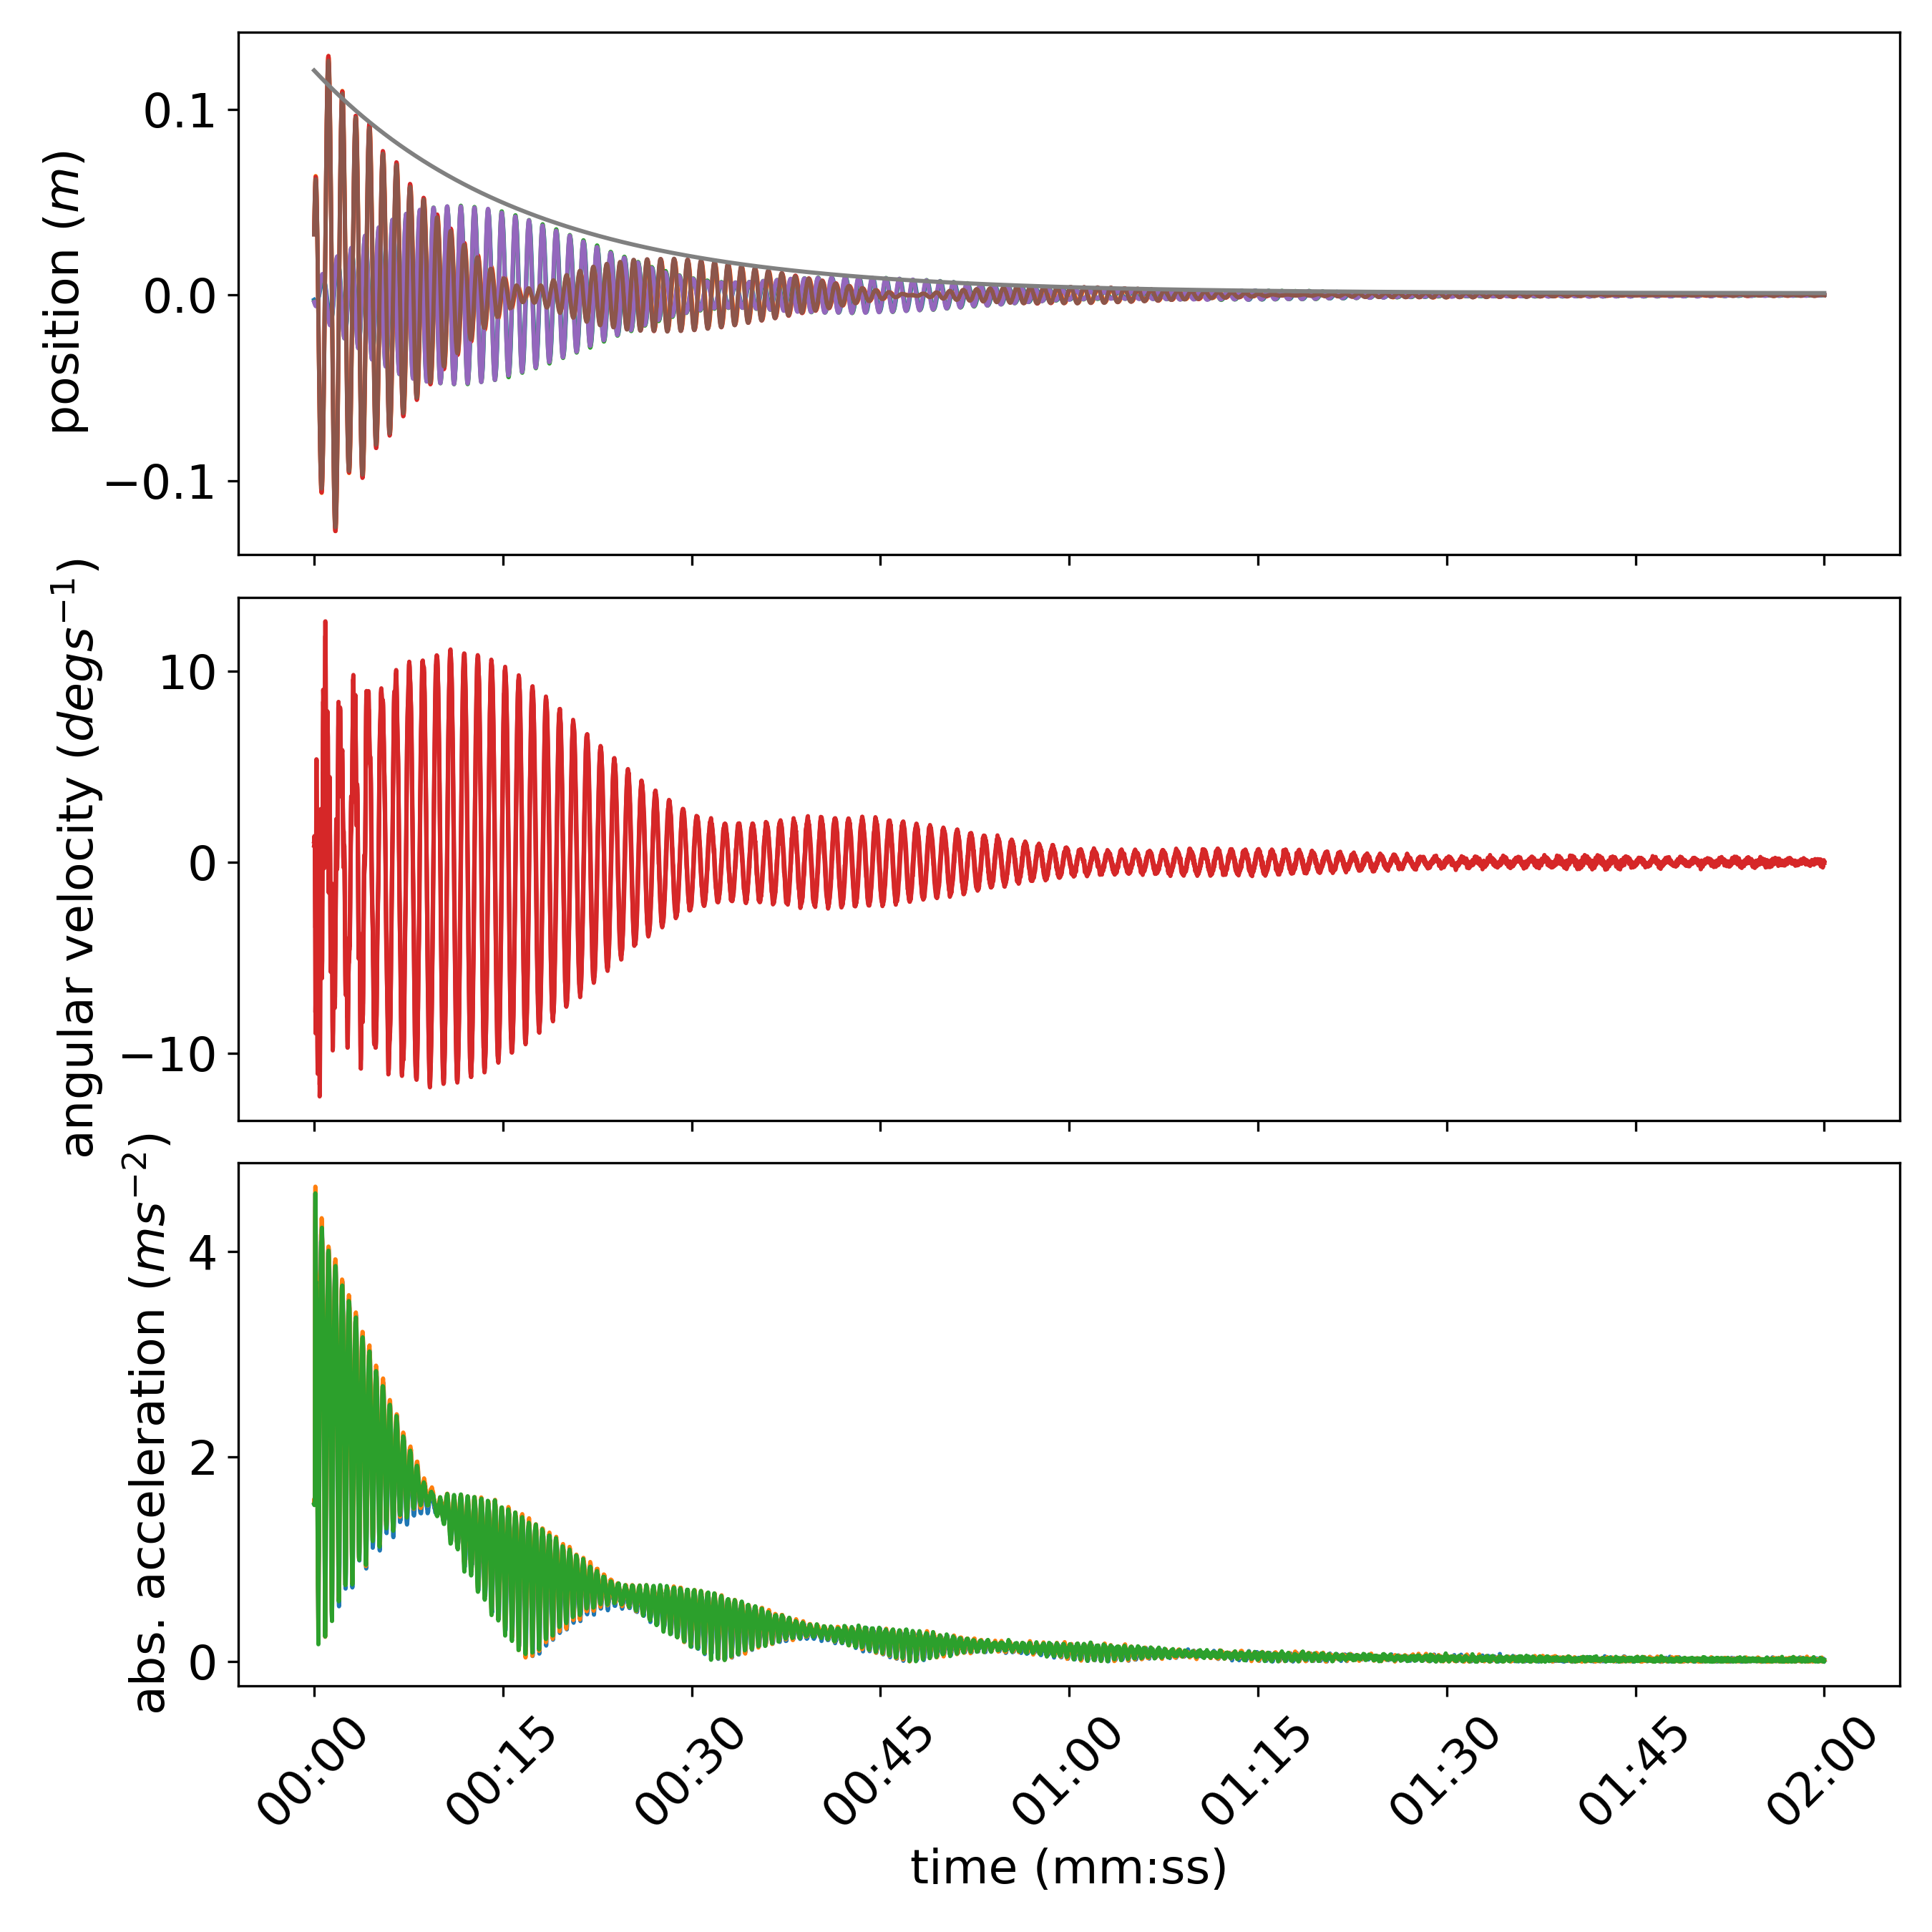
\includegraphics[width=\textwidth]{results/experiment/high_mass_acceleration.png}
        \caption{}
        % \caption{Scatter diagram for mean deflection $d_{10}$ and significant wave height $H_{S10}$. The linear fit is shown as a blue line.}
        \label{fig:high-mass:acc}
    \end{subfigure}
    \begin{subfigure}[b]{0.45\textwidth}
        \centering
        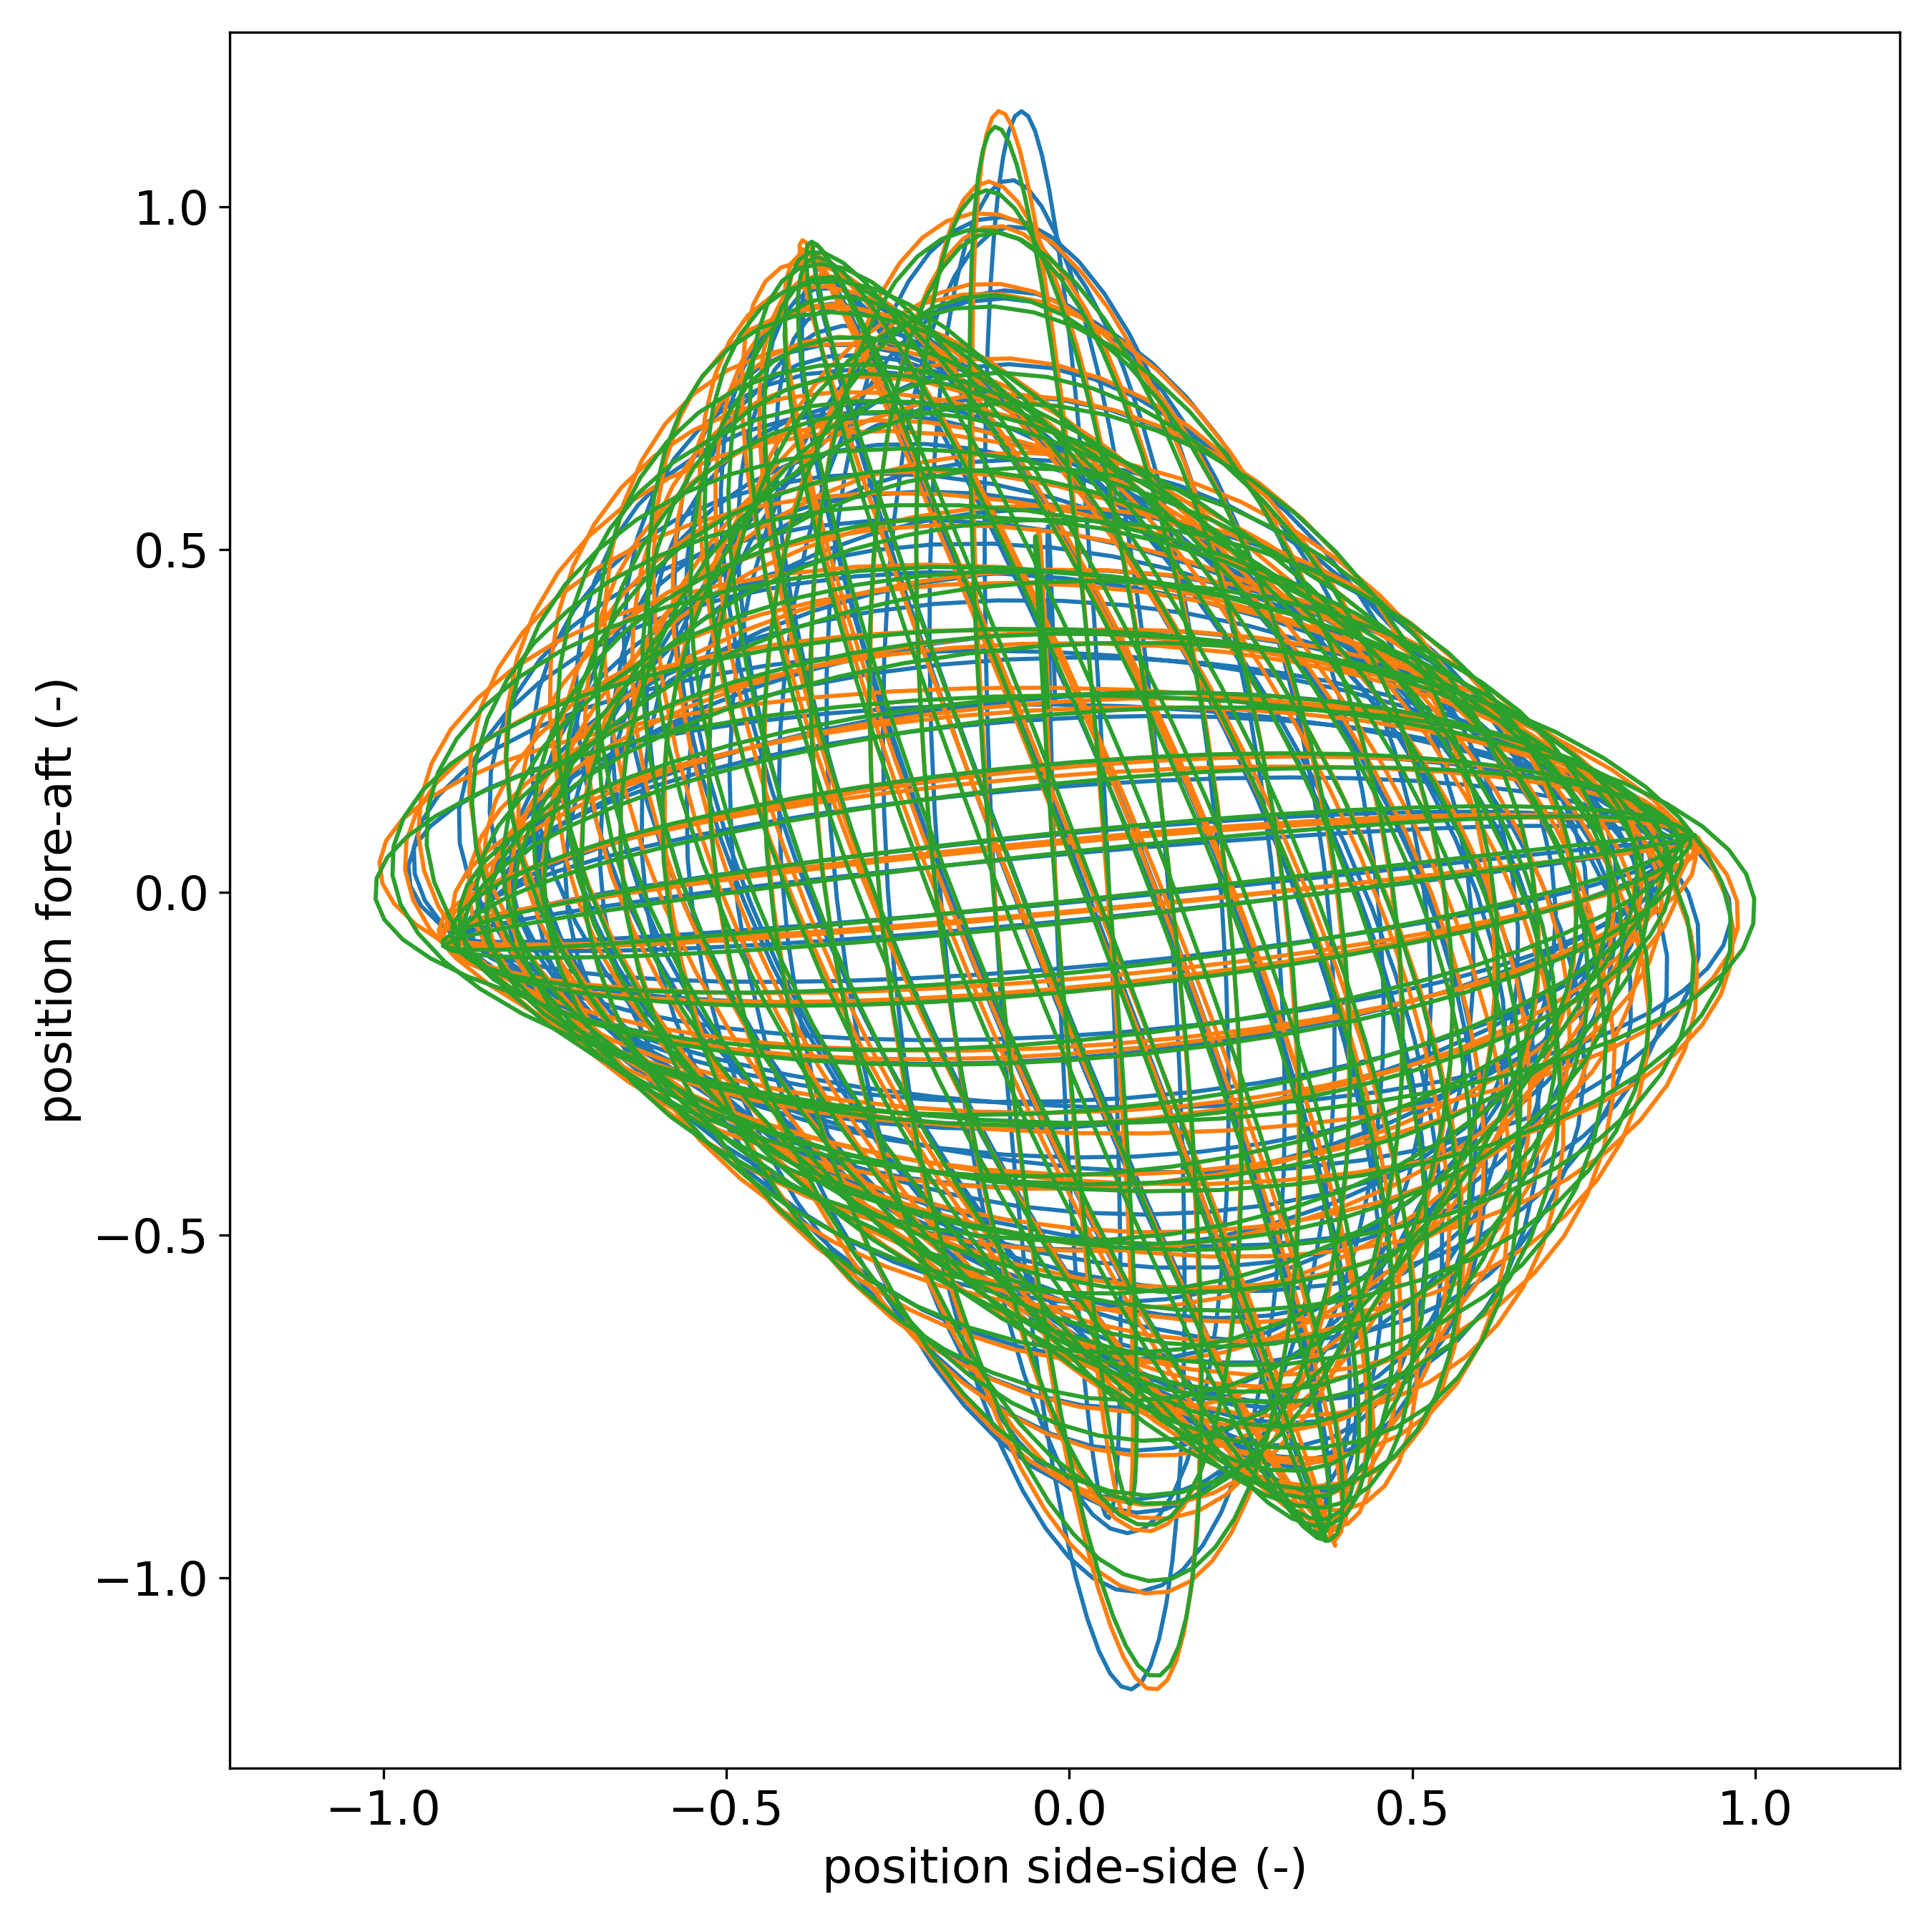
\includegraphics[width=\textwidth]{results/experiment/high_mass_orbit.png}
        \caption{}
        % \caption{Scatter diagram for mean deflection $d_{10}$ and significant wave height $H_{S10}$. The linear fit is shown as a blue line.}
        \label{fig:high-mass:orbit}
    \end{subfigure}
    
    
    \caption{Lissajous figures (orbits) for three different eccentric masses. \andy{[What are top's masses and moment of inertias of these configurations?]}}
    \label{fig:high-mass}
\end{figure*}

\begin{figure}
    \centering
    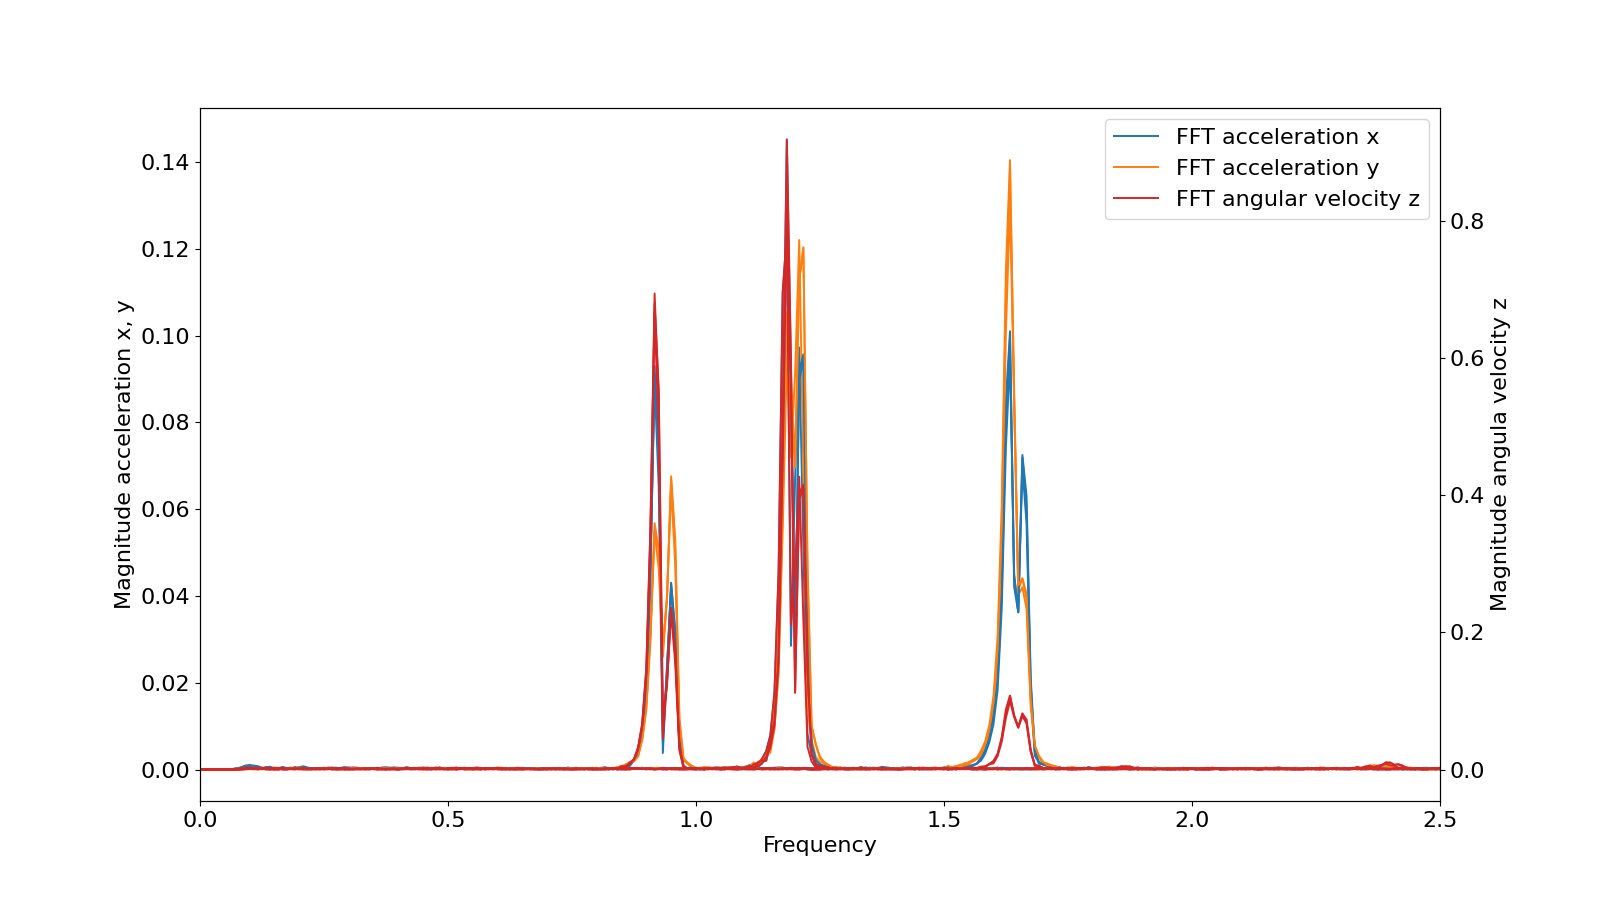
\includegraphics[width=0.5\linewidth]{results/experiment/spectrum.png}
    \caption{Caption}
    \label{fig:spectrum}
\end{figure}

\clearpage

% \section{Simulations (BAS)}
% \label{sec:simulations}

% \subsection{Simulation Setup}

% \paragraph{Model}
% A numerical model with six global degrees of freedom of the simplified system as shown in Figure \ref{fig:loading} was created. The support structure was modelled using linear one-dimensional finite element equations for undamped tension, torsion and bending of a cylinder with constant cross-section everywhere. Homogeneous linear elastic material was assumed and Euler Bernoulli beam theory was used for bending. The foundation was modelled with uncoupled springs, at the bottom of the support structure. 
% % \begin{small}(Eq.\ref{eq:fea:K_fnd})
% % \begin{equation}
% % \mathbf{K}_{fnd} =
% % \begin{bmatrix}
% % k_{x} &  &  &   &   &   \\ &  k_{y} &  &   &   &   \\ &   &  k_{z} &  & 0  &   \\ &   &   &  k_{\phi } &  &   \\ &   &   &   &  k_{\theta } &  \\ &   &   &   &   &  k_{\psi } 
% % \end{bmatrix}
% % \label{eq:fea:K_fnd}
% % \end{equation}
% % \end{small}
% The mass at the top of the structure was modelled as a concentrated mass with inertia, without eccentricity, and a point mass with eccentricity in both the horizontal and the vertical plane. The resulting mass matrix added to the top of the support structure is presented in Eq. \ref{eq:fea:Mtop}.
% \begin{small}
% \begin{equation}
% \mathbf{M}_{con.} + \mathbf{M}_{ecc.}  = 
% \begin{bmatrix}
%  m_{e}+m_{c} & 0 & 0 & 0 & m_{e}\,z_{e} & -m_{e}\,y_{e}\\ 0 & m_{e}+m_{c} & 0 & -m_{e}\,z_{e} & 0 & m_{e}\,x_{e}\\ 0 & 0 & m_{e}+m_{c} & m_{e}\,y_{e} & -m_{e}\,x_{e} & 0\\ 0 & -m_{e}\,z_{e} & m_{e}\,y_{e} & I_{c}+\left({z_{e}}^2+{y_{e}}^2\right)\,m_{e} & -m_{e}\,x_{e}\,y_{e} & -m_{e}\,x_{e}\,z_{e}\\ m_{e}\,z_{e} & 0 & -m_{e}\,x_{e} & -m_{e}\,x_{e}\,y_{e} & I_{c}+\left({z_{e}}^2+{x_{e}}^2\right)\,m_{e} & -m_{e}\,y_{e}\,z_{e}\\ -m_{e}\,y_{e} & m_{e}\,x_{e} & 0 & -m_{e}\,x_{e}\,z_{e} & -m_{e}\,y_{e}\,z_{e} & I_{c}+\left({y_{e}}^2+{x_{e}}^2\right)\,m_{e} 
% \end{bmatrix}
% \label{eq:fea:Mtop}
% \end{equation}
% \end{small}
% Taking gravity into account, the eccentricity of the top mass in the vertical plane introduces springs with  stiffness \(-g\,m_{e}\,z_{e}\) at top of the tower, for rotation about both horizontal axes and  the eccentricity of the top mass in the
% horizontal plane introduces static force and moments, presented wth Eq. \ref{eq:fea:Fstat}.
% \begin{small}
% \begin{equation}
% \mathbf{f}_g = 
% \begin{bmatrix}
%  0, & 0, & -g(\,m_{e}+m_{c}),& -g\,m_{e}\,y_{e}& g\,m_{e}\,x_{e},& 0
% \end{bmatrix}^{T}
% \label{eq:fea:Fstat}
% \end{equation}
% \end{small}
% The mass and stiffness of the system, equal to the summation of the mass and stiffness of the foundation, top mass and cylinder, has the form:
% \begin{equation}
% \mathbf{\bar{M}}\ddot{\mathbf{u}}+\mathbf{\bar{K}}\mathbf{u} = \mathbf{\bar{f}} 
% \end{equation}

% where \(\mathbf{\bar{M}} = \mathbf{M}_{cyl.}+\mathbf{M}_{conc.}+\mathbf{M}_{ecc.}\), $\mathbf{\bar{K}} = \mathbf{k}_{cyl}+\mathbf{K}_{ecc}+\mathbf{K}_{fnd}$ and  $\mathbf{\bar{f}} = \mathbf{f}_{g}+\mathbf{f}_{app}$.  








% A numerical model of the simplified system as shown in Figure \ref{fig:loading} was made, . The support structure was modelled with on linear one-dimensional finite element equations for tension, torsion and bending. Homogeneous linear elastic material was assumed and Euler Bernoulli beam theory was used for bending. It is assumed damping does not affect the formation of orbital motion and is thereby neglected, and thus the model can be described by \( \mathbf{M}\ddot{\mathbf{u}}+\mathbf{K}\mathbf{u} = \mathbf{F} \).
% The support structure is modelled as a vertical cylinder with constant cross-section. The foundation is modelled by six springs, one spring for each degree of freedom of the system. The eccentric mass is modelled as a cube with distributed mass, without eccentricity, and an additional eccentric point mass. The eccentricity and related coupling of the point mass is linearised and considered in the horizontal plane only (rotation about vertical axis), since for tower top motions of offshore wind turbines rotation about horizontal axes is assumed negligible. The resulting mass matrix for the distributed mass and eccentric point mass, added to the top node of the structural model, is presented below.
% \begin{equation}
%     M = 
% \end{equation}
% \begin{enumerate}
%     \item add mass matrix
% \end{enumerate}

% \paragraph{Loads}
% For the simulations,  initial deformation due to an horizontal force, applied at the centre of the top of the support structure, and gravitational force was considered. Multiple combinations of amplitude and direction of the initial deformation were considered, with and without gravitational force. In addition, the top mass and its eccentricity were varied. 

% % For the simulations, initial deformation and static load due to dead-weight were considered. No dynamic forces were applied. Initial deformations for two cases were obtained by applying force in the horizontal plane at the centre of the top of the model, with an angle of 90 degree and 85 degree witch respect to the eccentricity of the point mass. For each force orientation, a simulation with and simulation without gravity was done. 


% \subsection{Simulation Results}


% \begin{figure}
%     \centering
%     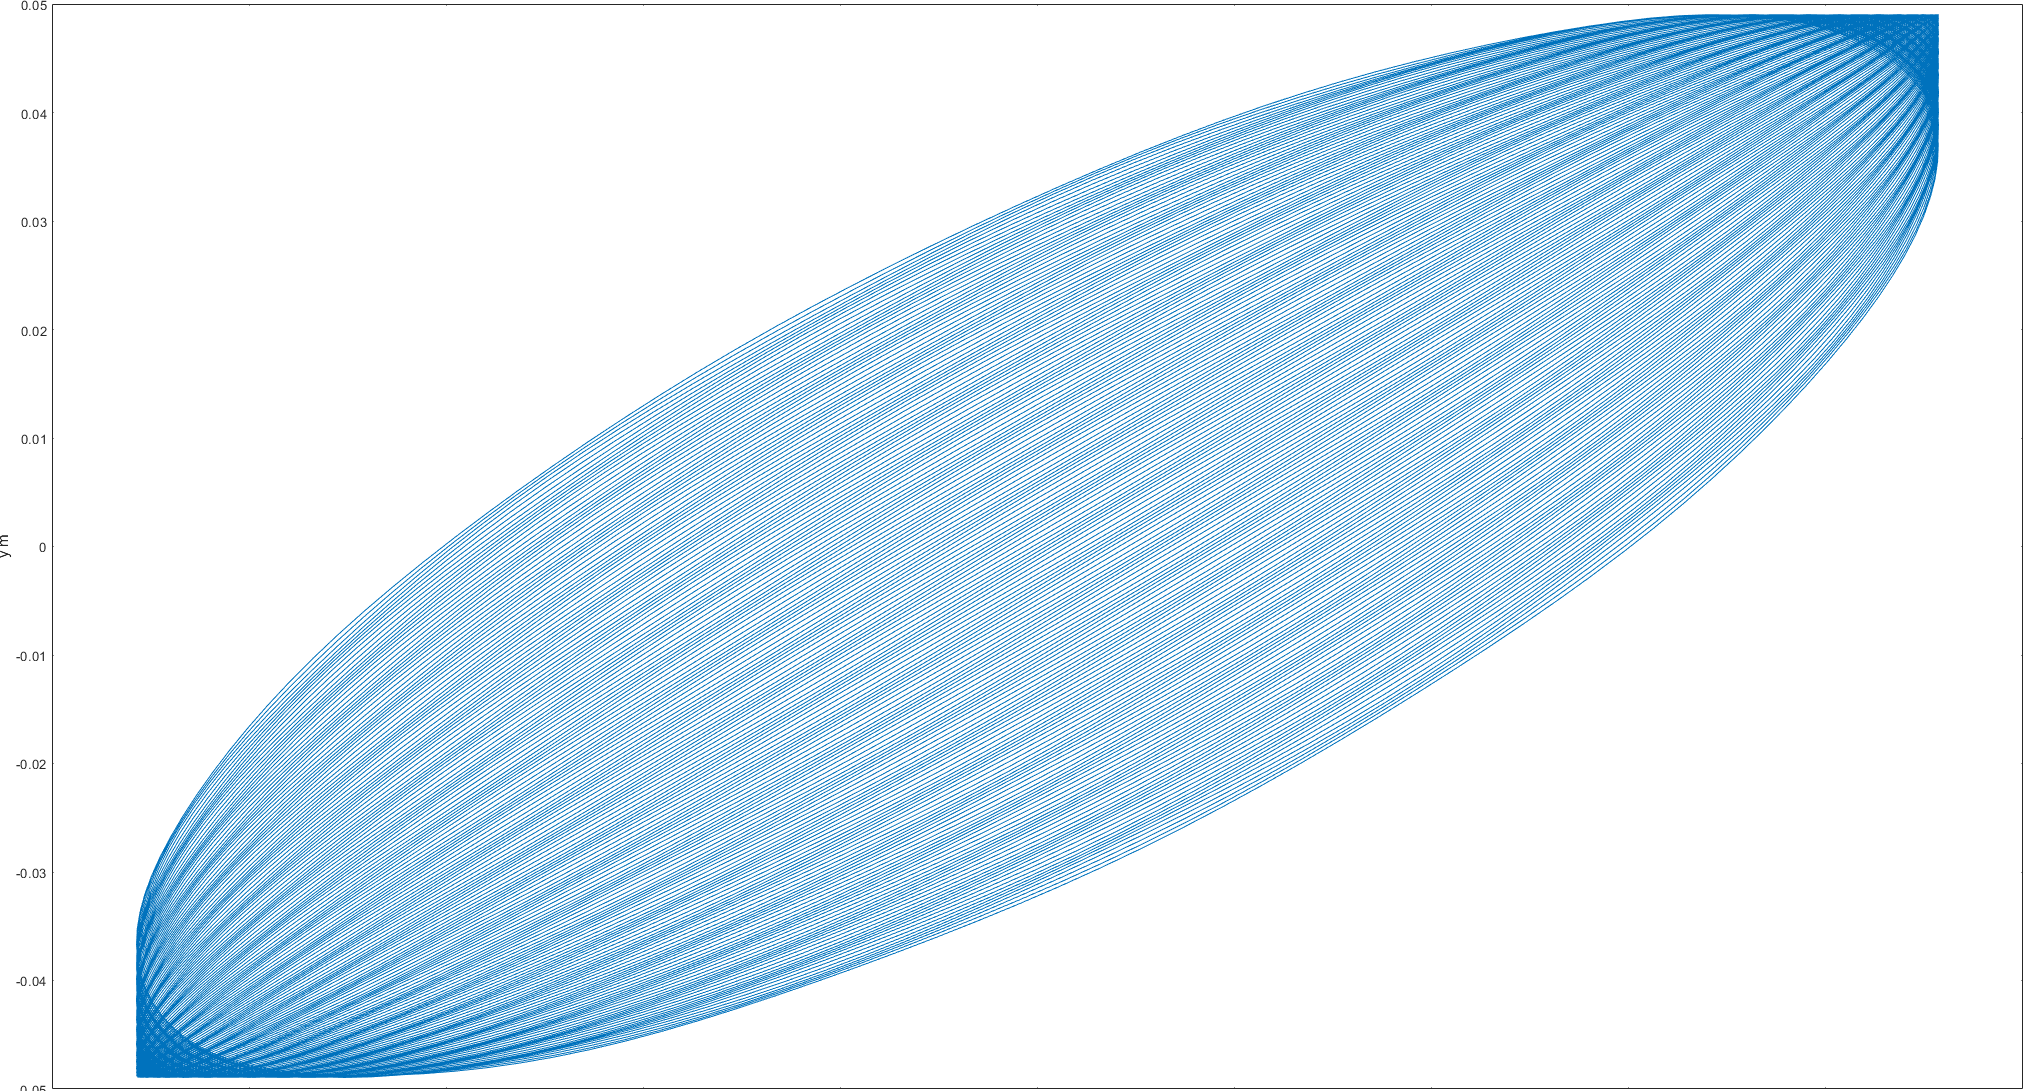
\includegraphics[width=0.5\linewidth]{manuscript/figures/Simulation_Orbits_LC__45degrees.png}
%     \caption{Orbits formation - without dead weight}
%     \label{fig:fea:45degrNograv}
% \end{figure}

% \begin{figure}
%     \centering
%     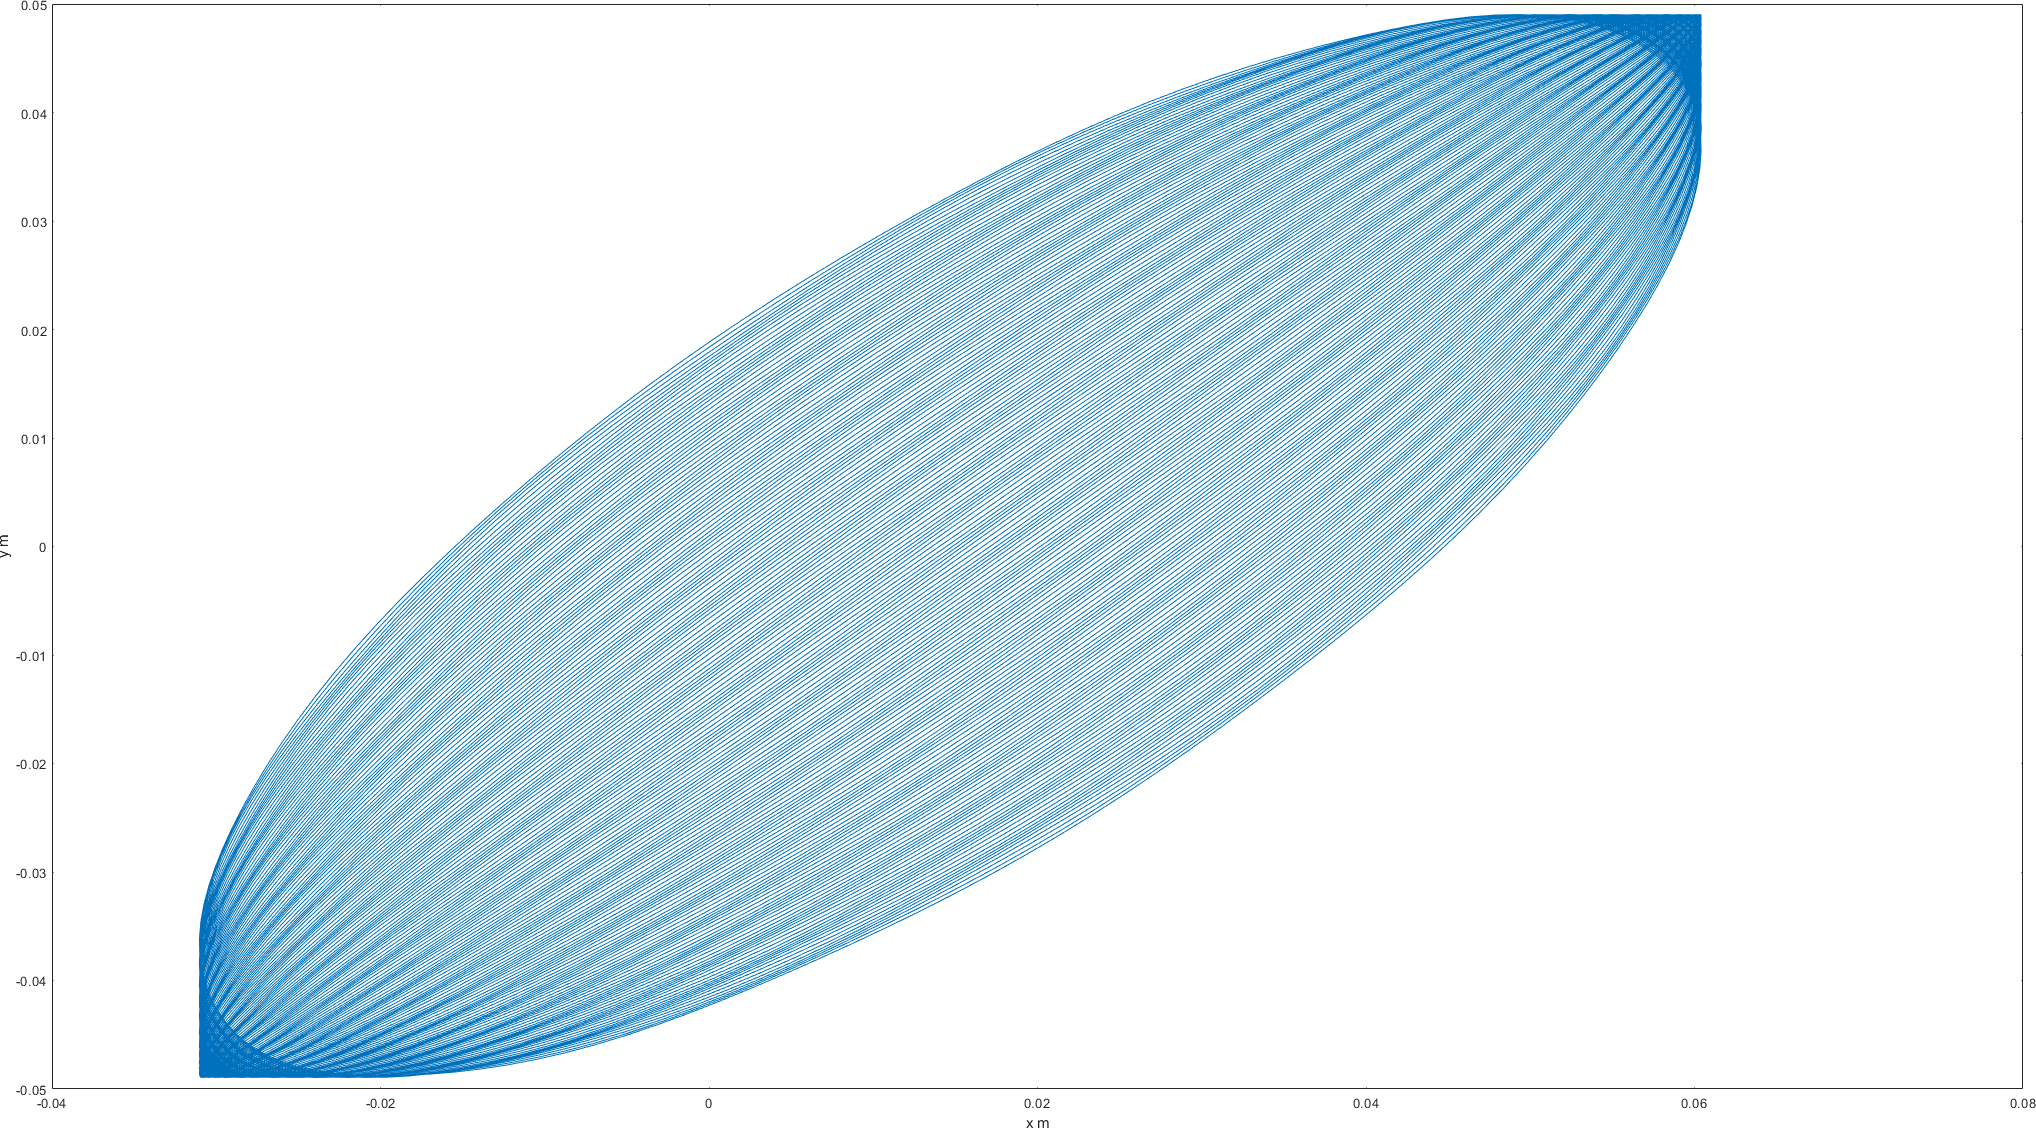
\includegraphics[width=0.5\linewidth]{manuscript/figures/Simulation_Orbits_LC__deadweight_45degrees.png}
%     \caption{Orbits formation - with dead weight}
%     \label{fig:fea:45degrWithgrav}
% \end{figure}
% \clearpage

\section{Simulations (BAS)}
\label{sec:simulations}

\subsection{Simulation Setup}

\paragraph{Model}
A numerical model based on the simplified system as shown in Figure \ref{fig:loading} was created using MATLAB, presented in Figure \ref{fig:fea:model}. The support structure was modelled as a hollow cylinder made of  homogeneous linear elastic material and with a constant cross-section along its length, supported by linear uncoupled springs. The nacelle was modelled as a concentrated mass with inertia and a point mass with eccentricity in both the horizontal and the vertical plane.
\begin{figure}[ht]
    \centering
    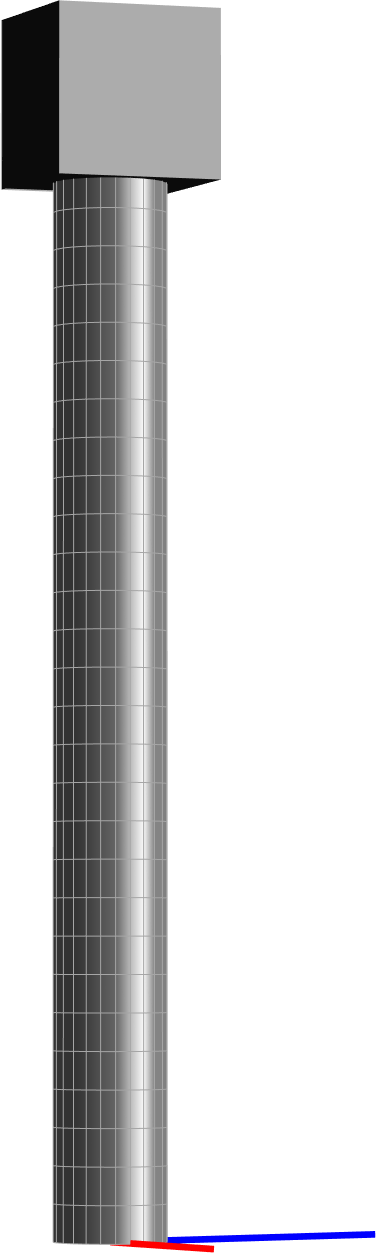
\includegraphics[width=0.7\linewidth]{manuscript/figures/FEModel.png}
    \caption{FE model}
    \label{fig:fea:model}
\end{figure}
The equations of motion of the undamped system, in the following form,
\begin{equation}
\mathbf{\bar{M}}\ddot{\mathbf{u}}+\mathbf{\bar{K}}\mathbf{u} = \mathbf{\bar{f}} 
\end{equation}
was obtained by superposition of the equations of motions of the concentrated and eccentric point mass, the support springs and the support structure. The support structure was modelled based on linear one-dimensional finite element equations for six degrees in the global coordinate system. Euler Bernoulli beam theory was used for bending. Using a rotation matrix based on Tait–Bryan angles, the equations of motions for the concentrated and eccentric top mass were derived with the Euler Lagrange equation. Using Taylor series for linearisation, the  mass matrix (Eq. \ref{eq:fea:Mtop}), stiffness matrix (Eq. \ref{eq:fea:K_m_ecc}) and gravitational force (Eq. \ref{eq:fea:Fstat}) were found for the six global degrees of freedom. The stiffness matrix of the support strings is presented in Eq. \ref{eq:fea:K_fnd}. 
\begin{small}
    \begin{equation}
        \mathbf{M}_{m_c} + \mathbf{M}_{m_e}  = 
        \begin{bmatrix}
         m_{e}+m_{c} & 0 & 0 & 0 & m_{e}\,z_{e} & -m_{e}\,y_{e}\\ 0 & m_{e}+m_{c} & 0 & -m_{e}\,z_{e} & 0 & m_{e}\,x_{e}\\ 0 & 0 & m_{e}+m_{c} & m_{e}\,y_{e} & -m_{e}\,x_{e} & 0\\ 0 & -m_{e}\,z_{e} & m_{e}\,y_{e} & I_{c}+\left({z_{e}}^2+{y_{e}}^2\right)\,m_{e} & -m_{e}\,x_{e}\,y_{e} & -m_{e}\,x_{e}\,z_{e}\\ m_{e}\,z_{e} & 0 & -m_{e}\,x_{e} & -m_{e}\,x_{e}\,y_{e} & I_{c}+\left({z_{e}}^2+{x_{e}}^2\right)\,m_{e} & -m_{e}\,y_{e}\,z_{e}\\ -m_{e}\,y_{e} & m_{e}\,x_{e} & 0 & -m_{e}\,x_{e}\,z_{e} & -m_{e}\,y_{e}\,z_{e} & I_{c}+\left({y_{e}}^2+{x_{e}}^2\right)\,m_{e} 
        \end{bmatrix}
        \label{eq:fea:Mtop}
    \end{equation}
\end{small}

\begin{small}
    \begin{equation}
        \mathbf{K}_{m_e} =
        \begin{bmatrix}
       0 &  &  &   &   &   \\ &  0 &  &   & 0  &   \\ &   &  0 &  &   &   \\ & &   &  -g\,m_{e}\,z_{e} &  &   \\ &   0  &   &   &  -g\,m_{e}\,z_{e} &  \\ &   &   &   &   &  0
        \end{bmatrix}
        \label{eq:fea:K_m_ecc}
    \end{equation}
\end{small}

\begin{small}
    \begin{equation}
        \mathbf{f}_{m_c} + \mathbf{f}_{m_e} = 
        \begin{bmatrix}
         0\\ 0\\ -g(\,m_{e}+m_{c})\\ -g\,m_{e}\,y_{e}\\ g\,m_{e}\,x_{e} \\ 0
        \end{bmatrix}
        \label{eq:fea:Fstat}
    \end{equation}
\end{small}

\begin{small}
    \begin{equation}
        \mathbf{K}_{fnd} =
        \begin{bmatrix}
        k_{x} &  &  &   &   &   \\ &  k_{y} &  &   & 0  &   \\ &   &  k_{z} &  &   &   \\ & &   &  k_{\phi } &  &   \\ &   0  &   &   &  k_{\theta } &  \\ &   &   &   &   &  k_{\psi } 
        \end{bmatrix}
        \label{eq:fea:K_fnd}
    \end{equation}
\end{small}

\paragraph{Loads }
Gravitational force and initial deformation due to an horizontal force applied at the centre of the top of the support structure were considered. Multiple combinations of amplitude and direction of the initial deformation were simulated, for load cases with and without gravitational force. In addition, the top mass and its vertical and horizontal eccentricity were varied.  To account for limitations due to linearization of the numerical model, small initial deformations were applied.

\subsection{Simulation Results}
The response to gravitational force and an initial deformation due to an horizontal force applied at the top of the  support structure with an angle of 45\textdegree with respect to the eccentricity of the point mass is presented in Figure \ref{fig:fea:lissa_simu_results}. The pattern in Figure  (\ref{fig:fea:lissa_orbits}),  similar to the pattern found with the experiments, as presented in Figure \ref{fig:high-mass:orbit}, can be described as a Lissajous curve. 

To compare the effect of gravitational force and vertical eccentricity of the point mass, the the response  for a load cases with- and without gravitational force and vertical eccentricity are presented in Figure \ref{fig:fea:simres_gravitational_force_comparison}. These responses result from simulations with a short time span and would have shown a similar pattern to the response presented in Figure\ref{fig:fea:lissa_simu_results}, (\ref{fig:fea:lissa_orbits}), if the simulation time span was extended. 

\begin{figure*}
\centering
    \begin{subfigure}[b]{0.45\textwidth}
        \centering
        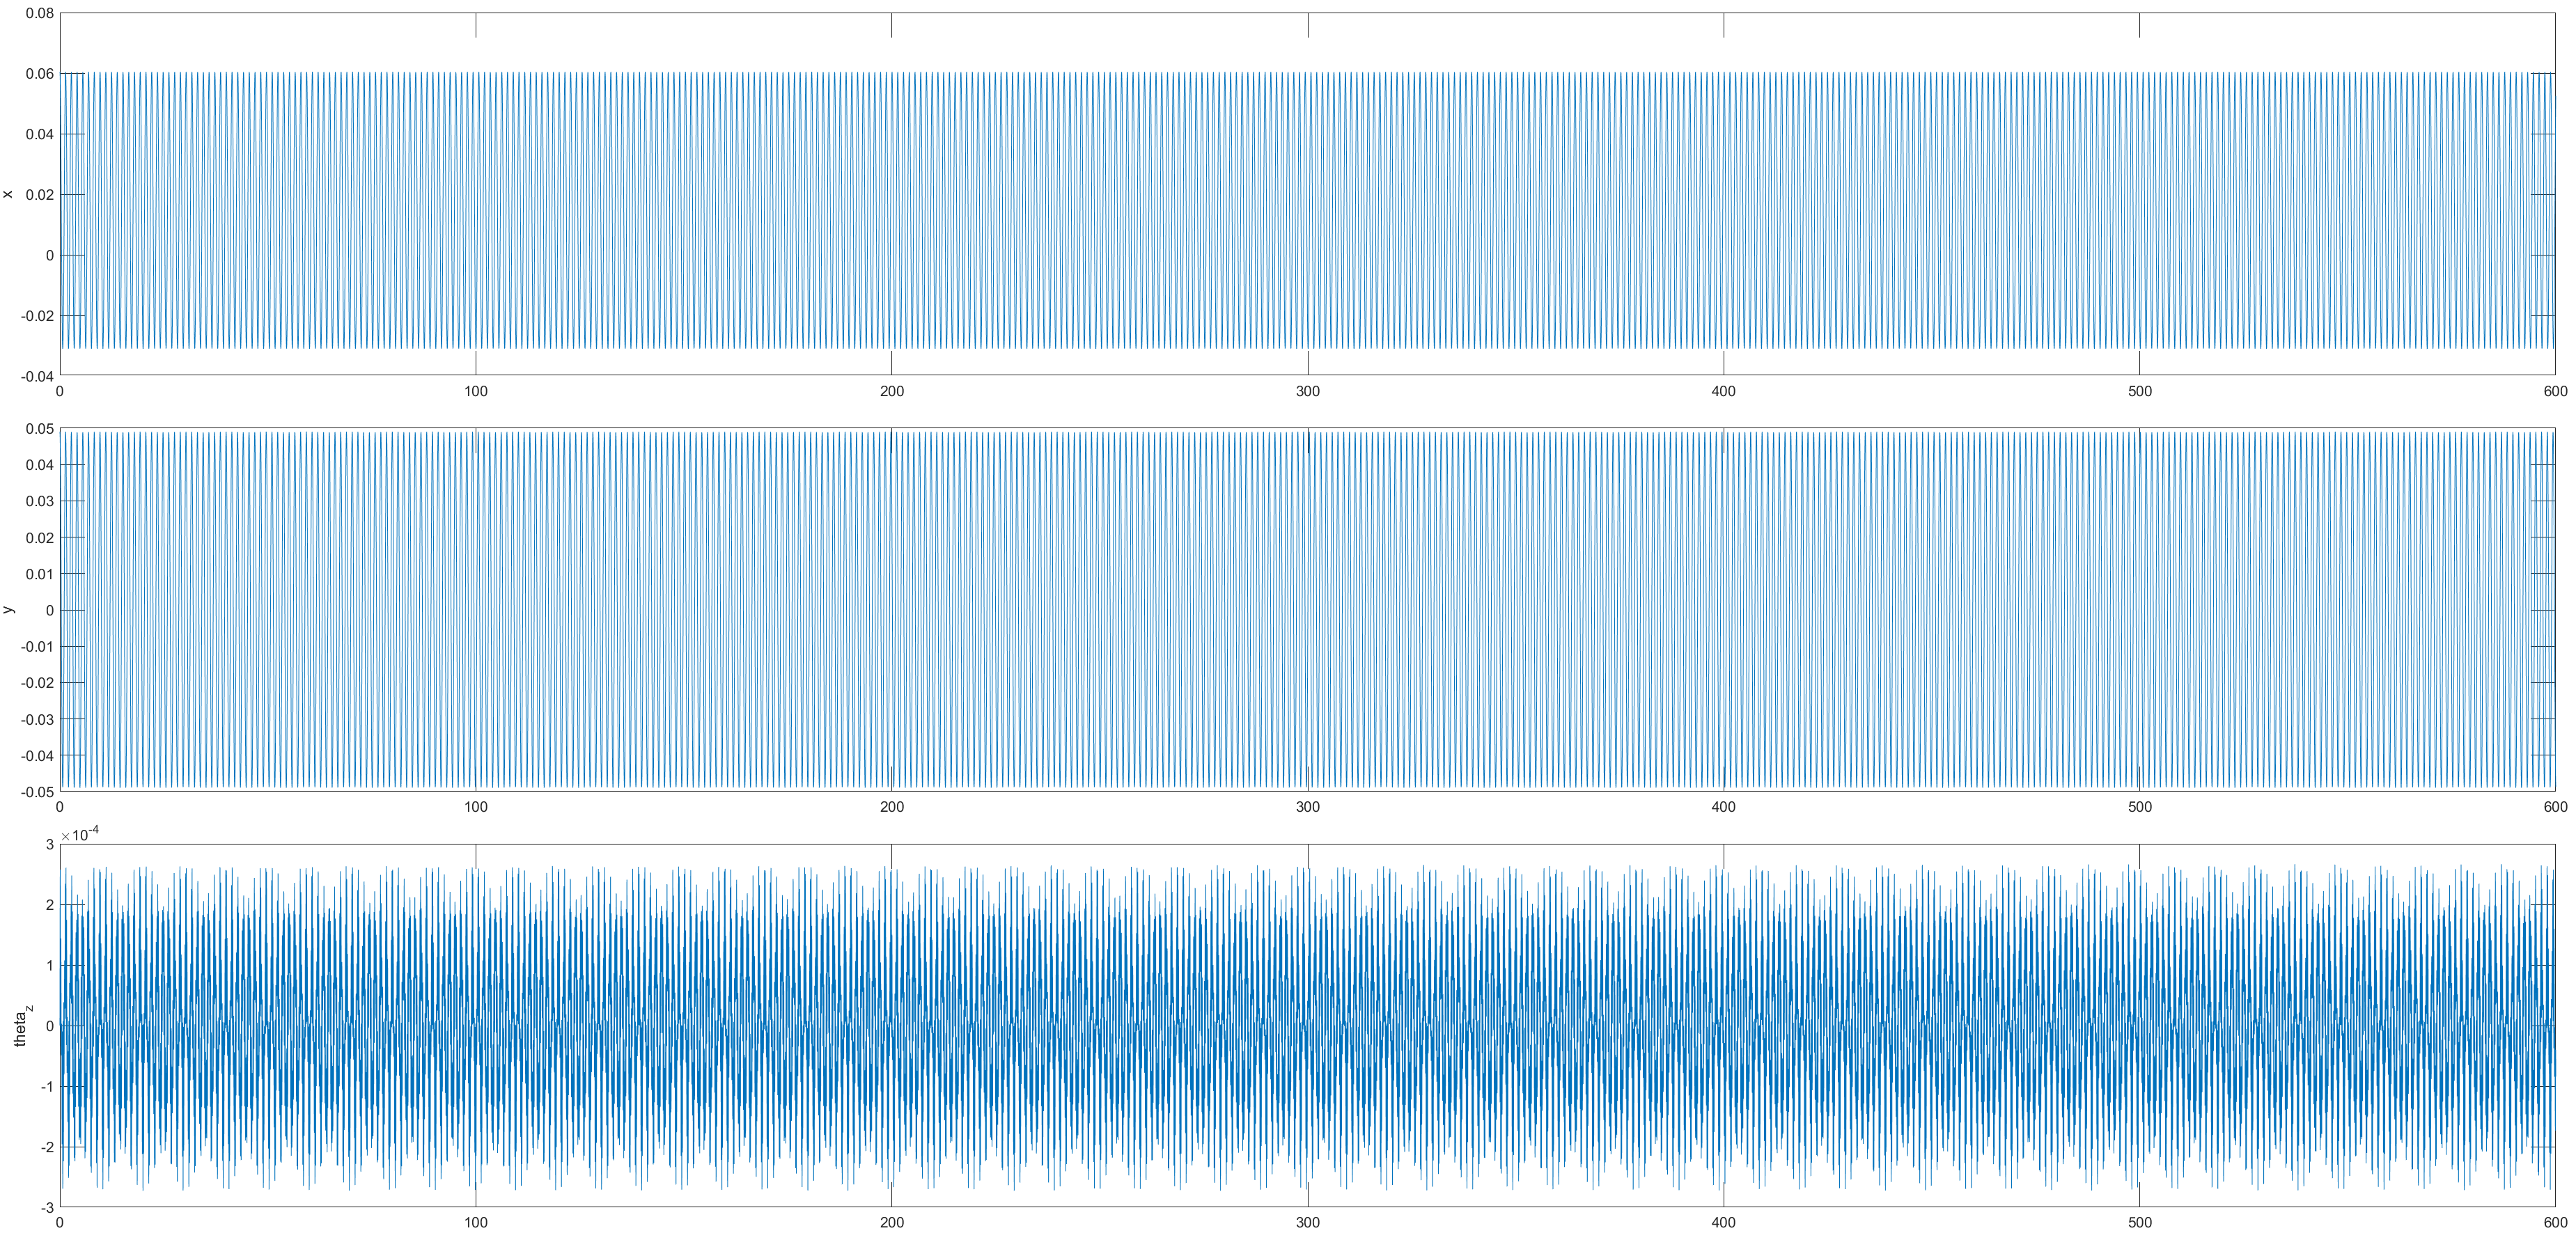
\includegraphics[width=\textwidth]{manuscript/figures/FEA_simu_Lissa_Displacement.png}
        % \caption{}
        % \caption{Scatter diagram for mean deflection $d_{10}$ and significant wave height $H_{S10}$. The linear fit is shown as a blue line.}
        \caption{\small{Horizontal displacement and rotation about vertical axis}}
        \label{fig:fea:lissa_displ}
    \end{subfigure}
    \begin{subfigure}[b]{0.45\textwidth}
        \centering
        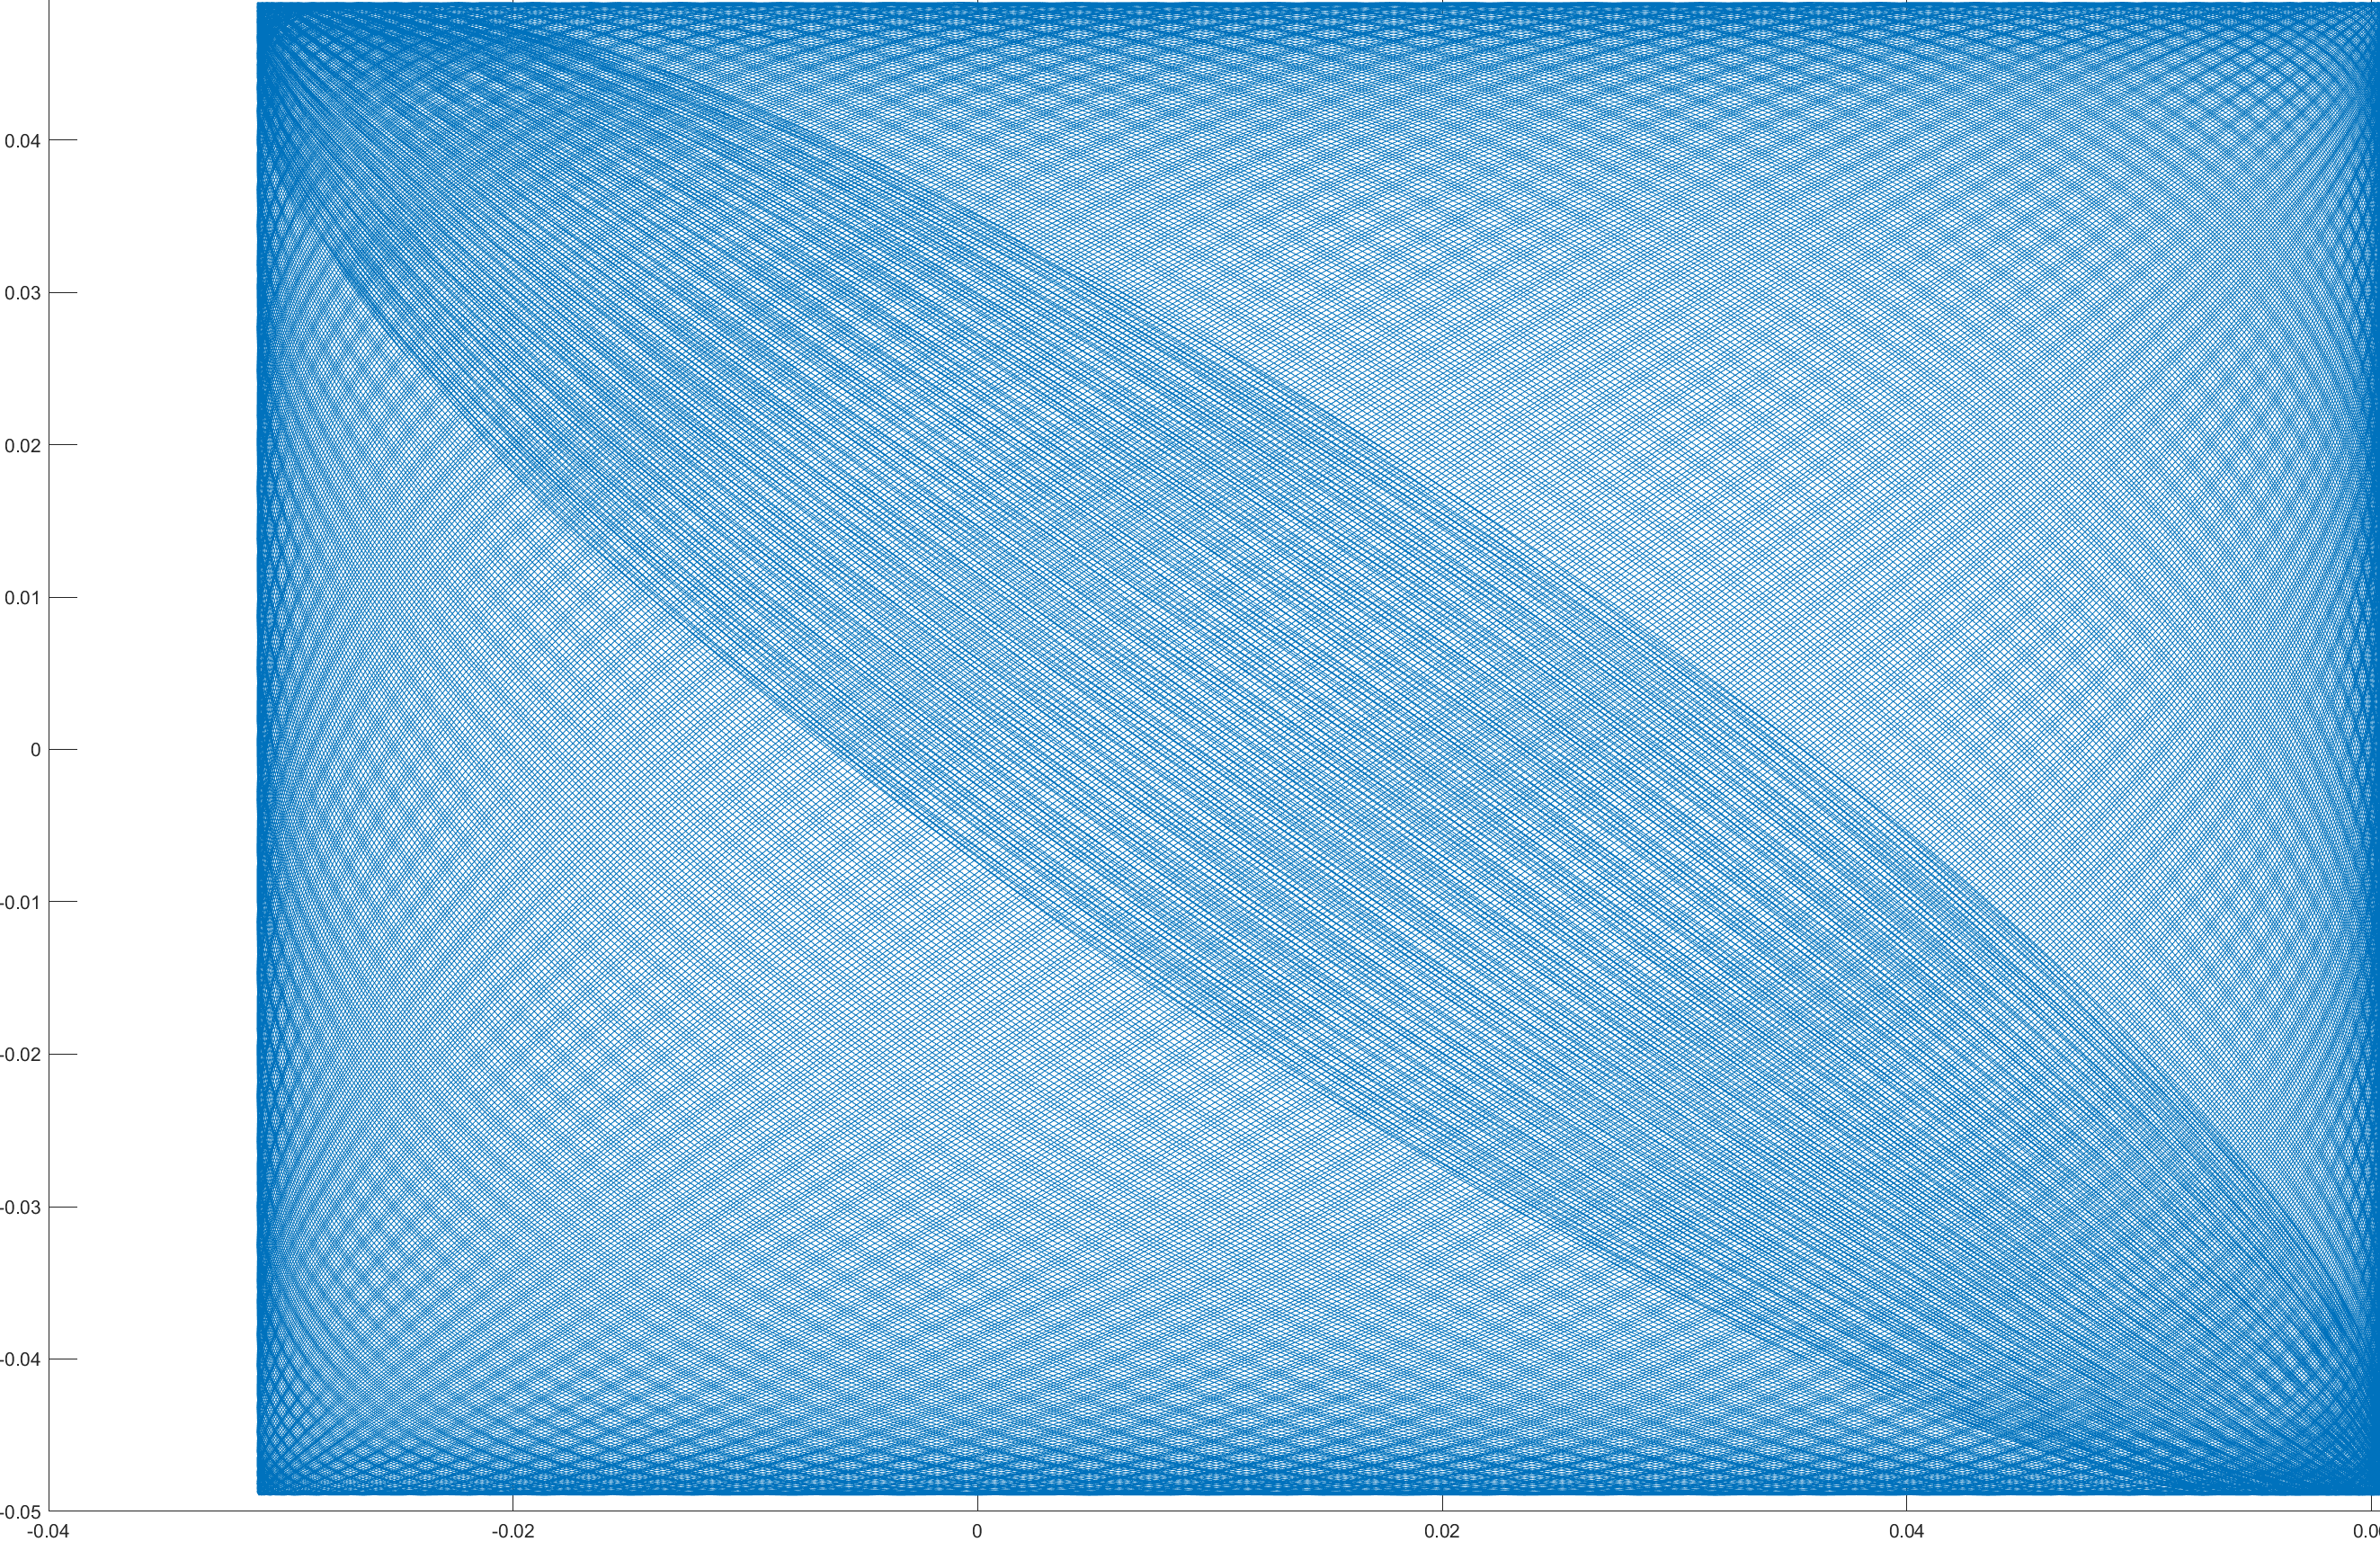
\includegraphics[width=\textwidth]{manuscript/figures/FEA_simu_Lissa_Orbits.png}
        \caption{\small{Formation of obits in the horizontal plane}}
        % \caption{Scatter diagram for mean deflection $d_{10}$ and significant wave height $H_{S10}$. The linear fit is shown as a blue line.}
        \label{fig:fea:lissa_orbits}
    \end{subfigure}
\caption{FE simulation results: Lissajous curve}
    \label{fig:fea:lissa_simu_results}
\end{figure*}


\begin{figure*}
\centering
    \begin{subfigure}[b]{0.45\textwidth}
        \centering
        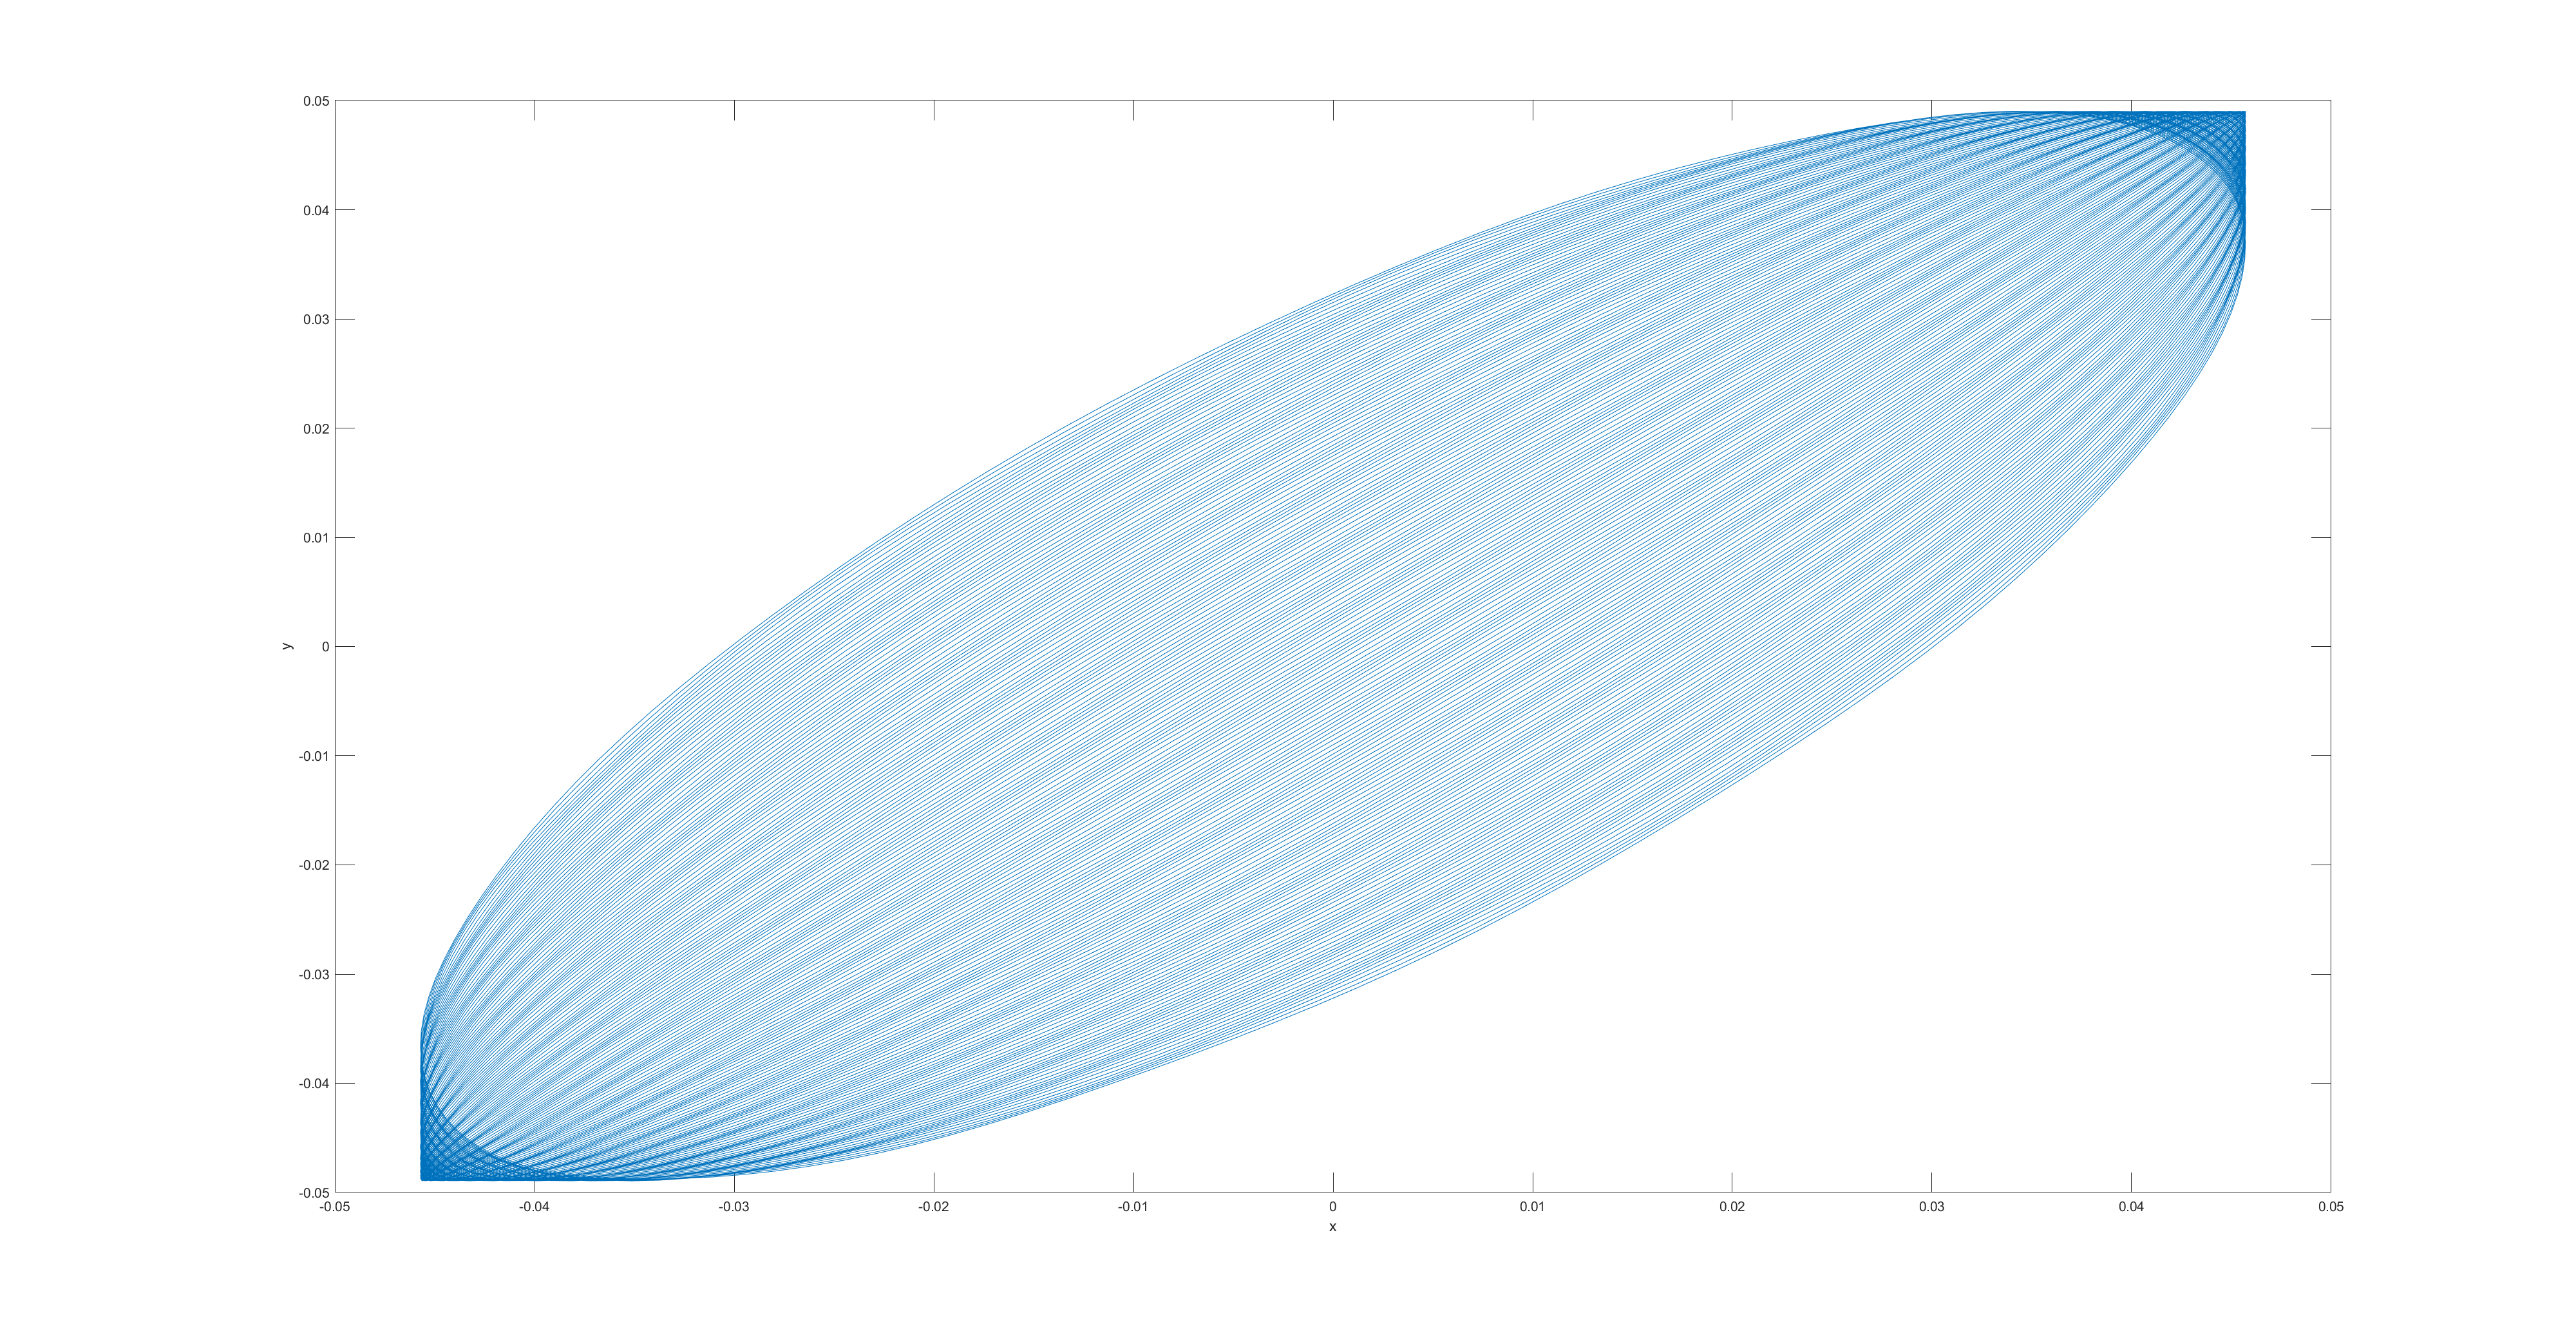
\includegraphics[width=\textwidth]{manuscript/figures/FEA_simu_Orbits_No_grav.png}
        % \caption{}
        % \caption{Scatter diagram for mean deflection $d_{10}$ and significant wave height $H_{S10}$. The linear fit is shown as a blue line.}
        \caption{\small{Without gravitational force}}
        \label{fig:fea:simres_nograp}
    \end{subfigure}
    \begin{subfigure}[b]{0.45\textwidth}
        \centering
        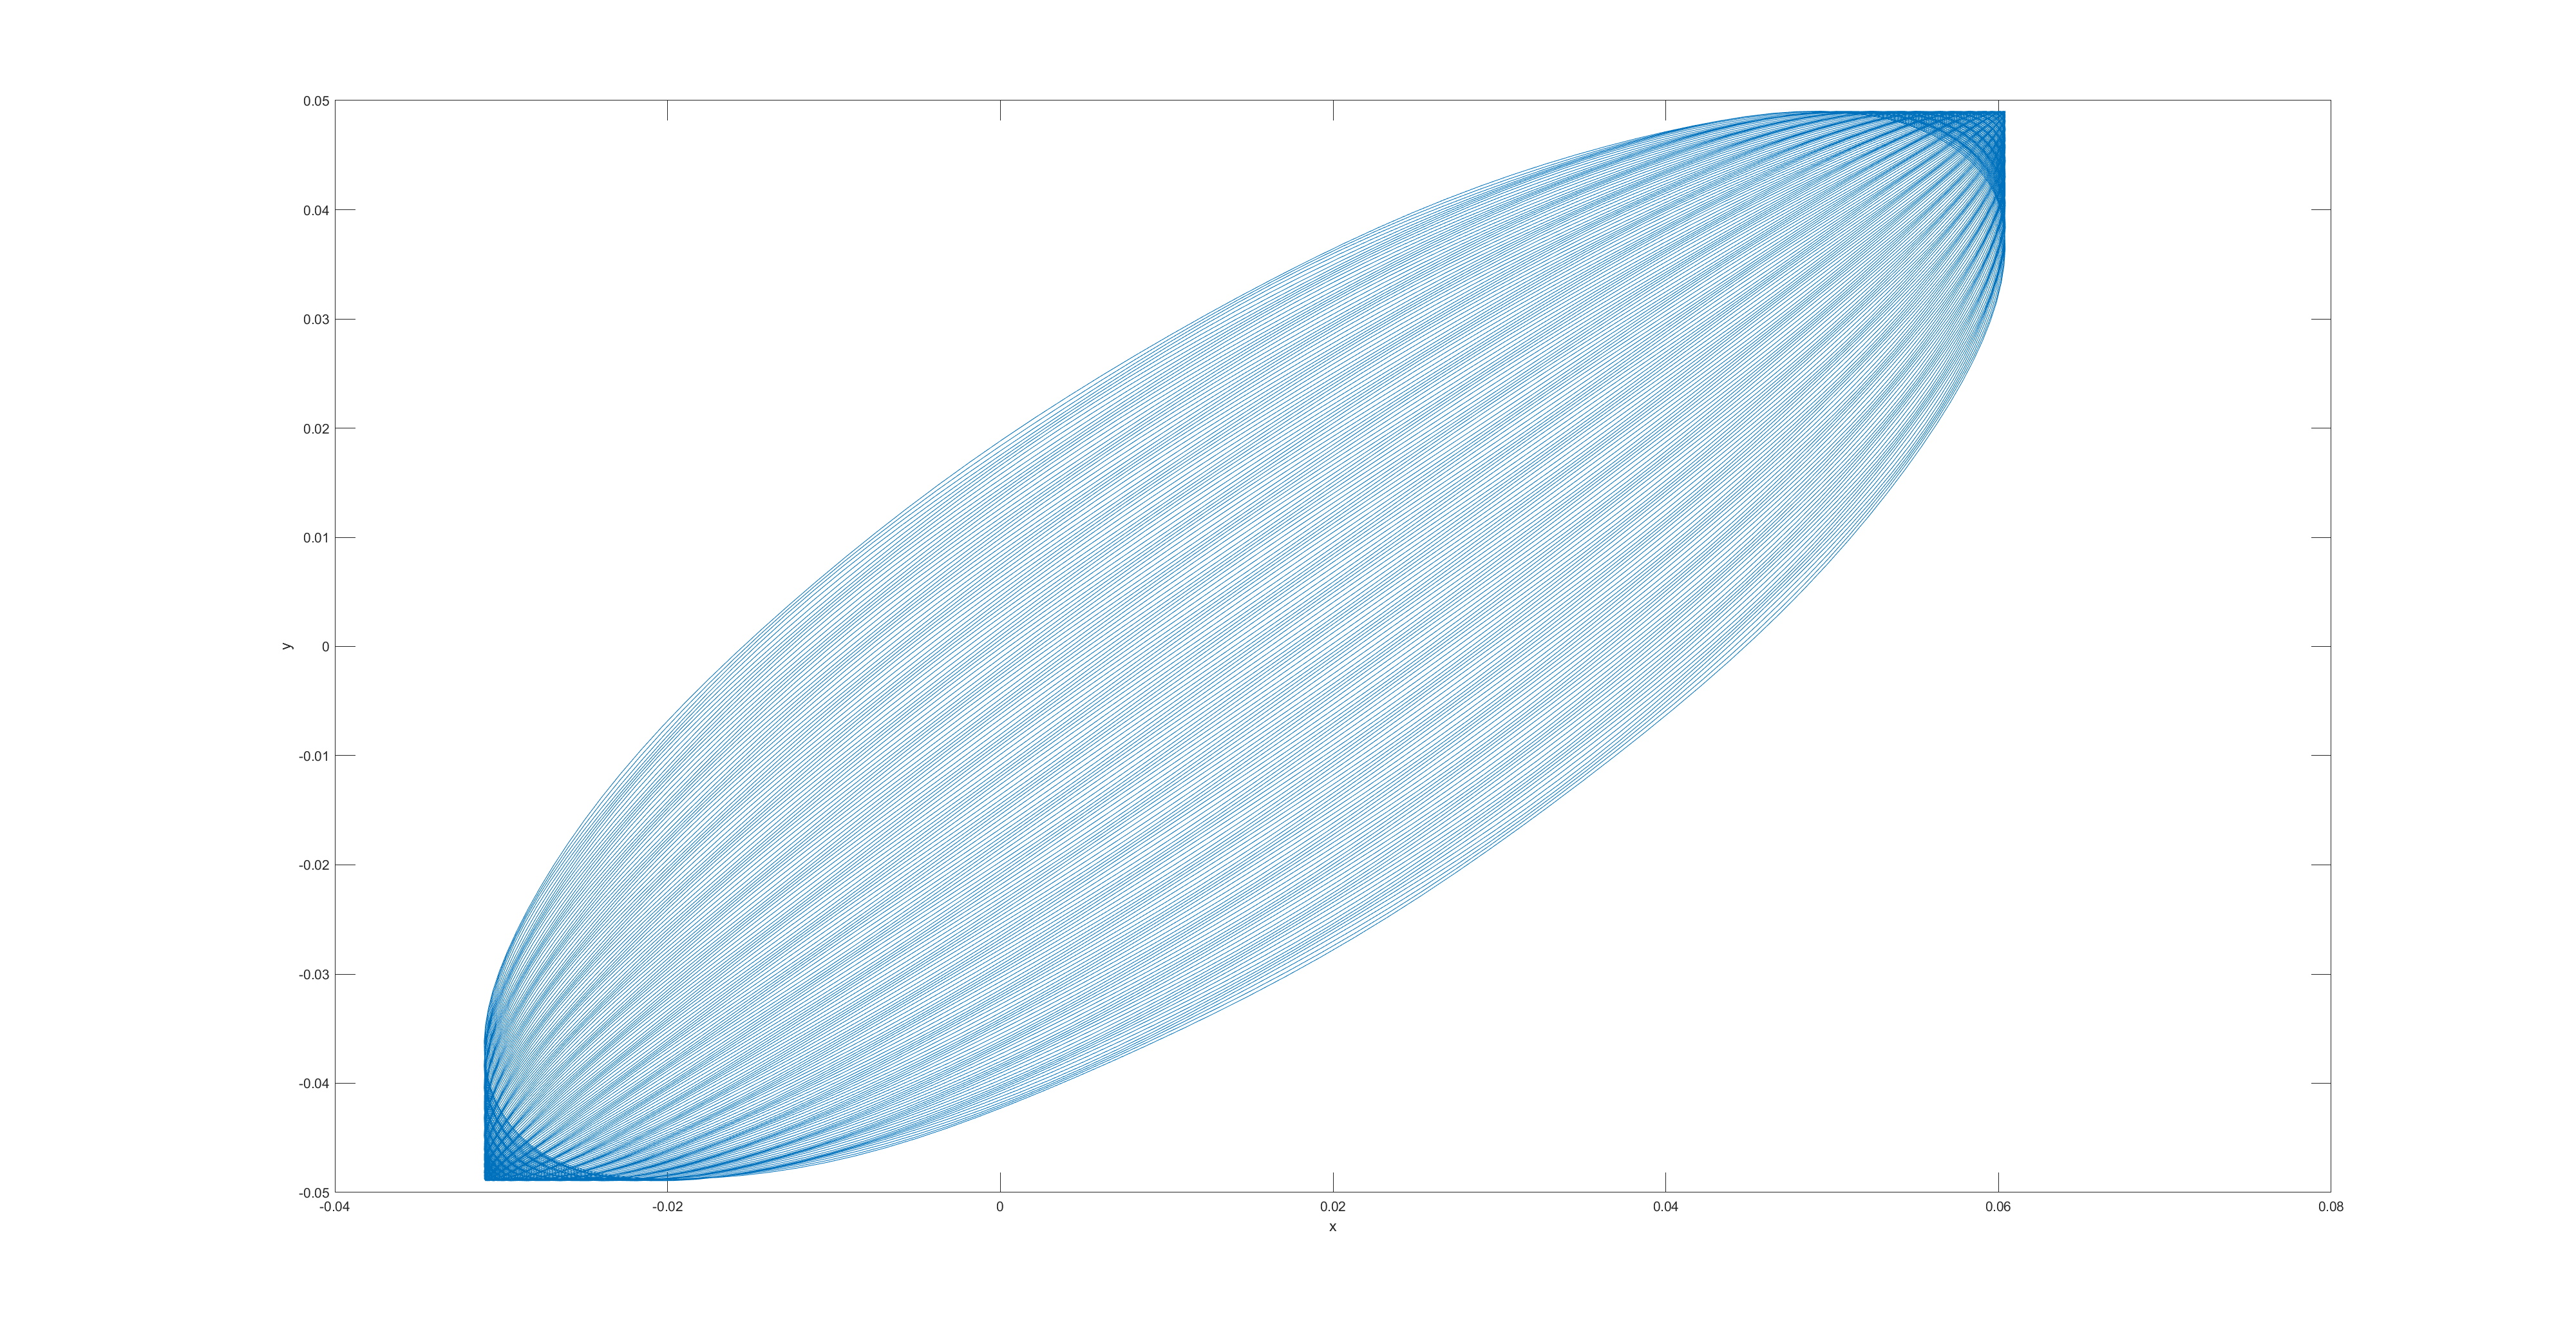
\includegraphics[width=\textwidth]{manuscript/figures/FEA_simu_Orbits_With_grav.png}
        \caption{\small{With gravitational force}}
        % \caption{Scatter diagram for mean deflection $d_{10}$ and significant wave height $H_{S10}$. The linear fit is shown as a blue line.}
        \label{fig:fea:simres_withgrav}
    \end{subfigure}
\caption{FE simulation results: with and without gravitational force}
    \label{fig:fea:simres_gravitational_force_comparison}
\end{figure*}

\clearpage

\section{A vibration model with three degrees of freedom}
\label{sec:3dof}

A common approach to study vibrations is to reduce the real system into a simplified model that consists of discrete components. In this approach, one aims to describe the real system as simple as possible to generate the main dynamics of the real system. Many vibration phenomena can be sufficiently described with systems with only one or two degrees of freedom. Here, we present a model with three degrees of freedom that seems to capture the main dynamics of the real system.
\par 
We model the real system in two dimensions (\autoref{fig:3dof-system}). The tower's bending is modelled as a linear spring, which is connected to a fixed point, which represents the tower's foundation, and to a first body, which represents the tower's top section. The tower's torsion is modelled with a torsional spring that connects a second body with a fixed angle in the inertial reference frame. This second body is pinned to the first body such that it translates with the first body, but rotates freely. Consequently, the system's three degrees of freedom are: the first body's position in $x$ and $y$ direction and the second body's orientation.
\par 
By applying the physical laws of conservation of linear and angular momentum, we derived the equations of motions for the system (a derivation is available as supplemental material). The system's equations of motion read:
\begin{equation}
    (m_1 + m_2) \ddot{x} - \cos(\theta) m_2 d \ddot{\theta} + \sin(\theta) m_2 d \dot{\theta}^2 + k_1 x = 0,\label{eq:eom-x}
\end{equation}
\begin{equation}
    (m_1 + m_2) \ddot{y} - \sin(\theta) m_2 d \ddot{\theta} - \cos(\theta) m_2 d \dot{\theta}^2 + k_1 y = 0,\label{eq:eom-y}
\end{equation}
\begin{equation}
    (I_{zz} + m_2 d^2)\ddot{\theta} - \cos(\theta) m_2 d \ddot{x} - \sin(\theta)m_2 d \ddot{y} + k_2 \theta = 0.\label{eq:eom-theta}
\end{equation}

The equations can be arranged to have only acceleration on the left hand side:
\begin{equation}
    \ddot{x} = \frac{1}{m_1 + m_2} \left( \cos(\theta) m_2 d \ddot{\theta} - \sin(\theta) m_2 d \dot{\theta}^2 - k_1 x \right),\label{eq:eom2-x}
\end{equation}
\begin{equation}
   \ddot{y} = \frac{1}{m_1 + m_2} \left(\sin(\theta) m_2 d \ddot{\theta} + \cos(\theta) m_2 d \dot{\theta}^2 - k_1 y \right),\label{eq:eom2-y}
\end{equation}
\begin{equation}
    \ddot{\theta} = \frac{1}{I_{zz} + m_2 d^2} \left(\cos(\theta) m_2 d \ddot{x} + \sin(\theta)m_2 d \ddot{y} - k_2 \theta \right) \label{eq:eom2-theta}
\end{equation}

Several terms couple translation ($x$ and $y$) with rotation ($\theta$): for example, the acceleration in the $x$ direction, $\ddot{x}$ is equal to terms that contain $\ddot{\theta}$ and $\dot{\theta}$ (\autoref{eq:eom2-x}). Such coupling terms are necssary to appear in the equation as otherwise only linear motion would be possible -- in other words, the mass would move back and forth on a straight line.
\par 
The translational acceleration is affected by the second mass' centrifugal and Euler forces. Centrifugal force acts in the $-\hat{r}$ direction and reads, 
\begin{equation}
    m_2 d \dot{\theta}^2,
\end{equation}
and Euler force acts in the $\hat{\theta}$ direction and reads
\begin{equation}
    m_2 d \ddot{\theta}.
\end{equation}
The equation for $\ddot{\theta}$ (\autoref{eq:eom2-theta}) was derived by applying conservation of angular momentum around the center of mass $G$. The force that acts at the location where the second body is pinned to the first body depend on the first body's acceleration in $x$ and $y$ direction such that there are also coupling terms with $\ddot{x}$ and $\ddot{y}$ in the equation for $\ddot{\theta}$  (\autoref{eq:eom2-theta}).
\par 
As expected, the equations also show that if $d=0$ the coupling terms disappear:
\begin{equation}
    (m_1 + m_2) \ddot{x} = - k_1 x,
\end{equation}
\begin{equation}
   (m_1 + m_2) \ddot{y} = - k_1 y,
\end{equation}
\begin{equation}
    I_{zz}\ddot{\theta} = - k_2 \theta.
\end{equation}

\begin{figure}
    \centering
    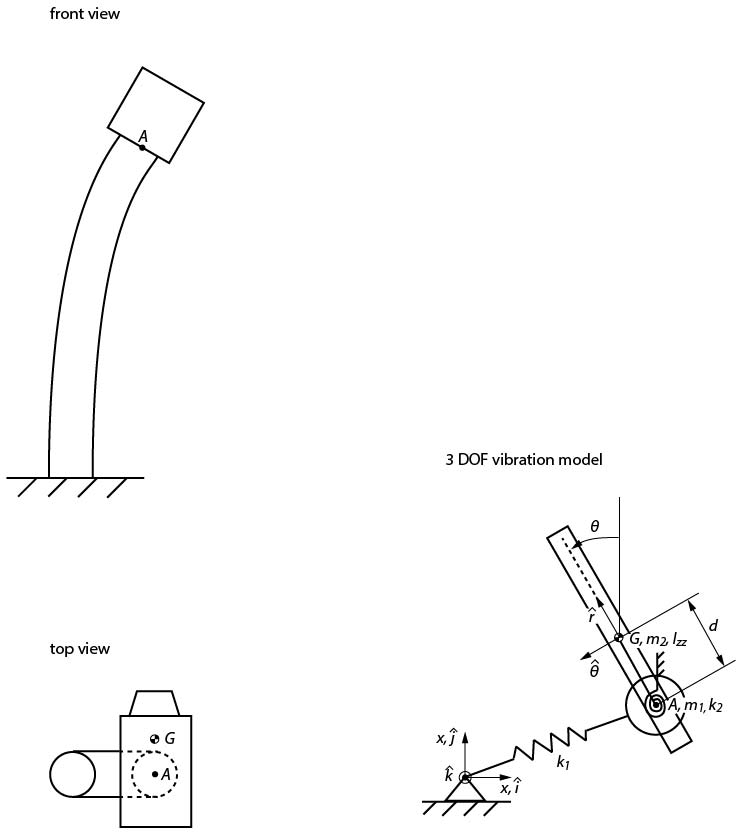
\includegraphics{manuscript/figures/vibration_model.jpg}
    \caption{A vibration model with three degrees of freedom (DOF).}
    \label{fig:3dof-system}
\end{figure}

The vibration model can reproduce the type of motions that were measured in the table top experiment and in the offshore measurement campaign [??? maybe the offshore measurements not]. \autoref{tab:3dof-variable-values} lists the parameter values that were estimated from the table top experiment and the offshore measurement campaign.

\begin{table}[]
    \centering
    \begin{tabular}{l l l l}
    \toprule
         Quantity & Table top experiment & Offshore measurements & Unit \\
         \midrule
         $m_1$ & 0.0093 & 320$\times$10$^3$ & kg\\ 
         $m_2$ & \{X, 0.044, X\} & 450$\times$10$^3$ & kg\\ 
         $k_1$ & 4.5 & 3.4$\times$10$^6$ & N\,m$^{-1}$ \\ 
         $k_2$ & 0.001 & 3.6$\times$10$^9$ & Nm\,deg$^{-1}$ \\ 
         $d$ & \{X, 0.038, X\} & 0.28 & m\\ 
         $I_{zz}$ & \{X, 5$\times$10$^{-5}$, X\} & 3.6$\times$10$^7$ & kg\,m$^2$ \\ 
         $\sqrt(x_0^2 + y_0^2)$ & 0.135 & - & m\\
         \bottomrule
    \end{tabular}
    \caption{Values used in the 3-DOF vibration model that correspond to the table top experiment and the offshore measurements.}
    \label{tab:3dof-variable-values}
\end{table}

\clearpage

\section{Discussion (ALL)}
\label{sec:discussion}

\subsection{Simulation}
With the linear numerical model, similar response patterns can be found to the patterns found with the experiments. The experiments were performed for initial deformations associated with geometrical non-linear effects which are not accounted for by the numerical model. Similar response patterns were obtained with the experiments and simulations, which indicates that the geometrical non-linear effects can be neglected. Simulations for load cases with- and without gravitational force and vertical eccentricity of point mass were performed, for eccentricity up to one thirtieth of the height of the support structure. The effect of  gravitational force and vertical eccentricity appeared negligible. Thereby, it is expected that a simple model with three degrees of freedom, namely translation in both horizontal direction and rotation in the horizontal plane, can be used instead of the rather complex FE model with six global degrees of freedom.


\begin{itemize}
    \item [Experiment]
    \begin{itemize}
        \item Initial and boundary conditions are hard to control. Experiment is sensitive to rod's orientation with respect to gravity. 
        \item more thorough parameter variation needed
        \item higher precision... 
    \end{itemize}
    \item [FE Simulations]
    \begin{itemize}
        \item 
    \end{itemize}
    \item [3 DoF Model]
    \begin{itemize}
        \item Numerical scheme
        \item Initial and boundary conditions estimated from the experiment do not yield the same orbits
        \item parameter study is needed
        \item Rigorous mathematical derivation to get from a cantileverd beam formulation (Bernoulli? Timoshenkov?) to a 3 DoF model.
    \end{itemize}
    \item[Overall]
    \begin{itemize}
        \item In all three approaches the orbits can be reproduced
        \item Orbit shapes compare, initial and boundary conditions do not
        \item Coupling effect is there, however: does it compare with offshore wind turbines?
    \end{itemize}
\end{itemize}

\clearpage

\bibliographystyle{unsrtnat}
\bibliography{references}  %%% Uncomment this line and comment out the ``thebibliography'' section 

\end{document}
